%%%%%%%% ICML 2026 EXAMPLE LATEX SUBMISSION FILE %%%%%%%%%%%%%%%%%

\documentclass{article}

% Recommended, but optional, packages for figures and better typesetting:
\usepackage{microtype}
\usepackage{graphicx}
\usepackage{subcaption}
\usepackage{booktabs} % for professional tables
\usepackage{siunitx}
% hyperref makes hyperlinks in the resulting PDF.
% If your build breaks (sometimes temporarily if a hyperlink spans a page)
% please comment out the following usepackage line and replace
% \usepackage{icml2026} with \usepackage[nohyperref]{icml2026} above.
\usepackage{hyperref}

\usepackage{adjustbox}
% Attempt to make hyperref and algorithmic work together better:
\newcommand{\theHalgorithm}{\arabic{algorithm}}

% % Use the following line for the initial blind version submitted for review:
% \usepackage{icml2026}

% For preprint, use
\usepackage{icml2026}

% If accepted, instead use the following line for the camera-ready submission:
% \usepackage{icml2026}

\usepackage{amsmath}
\usepackage{amssymb}
\usepackage{mathtools}
\usepackage{amsthm}
\usepackage{booktabs}
\usepackage{makecell}
\usepackage{multirow}
% if you use cleveref..
\usepackage[capitalize,noabbrev]{cleveref}

%%%%%%%%%%%%%%%%%%%%%%%%%%%%%%%%
% THEOREMS
%%%%%%%%%%%%%%%%%%%%%%%%%%%%%%%%
\theoremstyle{plain}
\newtheorem{theorem}{Theorem}[section]
\newtheorem{proposition}[theorem]{Proposition}
\newtheorem{lemma}[theorem]{Lemma}
\newtheorem{corollary}[theorem]{Corollary}
\theoremstyle{definition}
\newtheorem{definition}[theorem]{Definition}
\newtheorem{assumption}[theorem]{Assumption}
\theoremstyle{remark}
\newtheorem{remark}[theorem]{Remark}

\newcommand{\chen}[1]{{\color{red}{\bf{Chen says:}} \emph{#1}}}
\renewcommand{\arraystretch}{0.95}
\setlength{\parskip}{0.35em}
% Todonotes is useful during development; simply uncomment the next line
%    and comment out the line below the next line to turn off comments
%\usepackage[disable,textsize=tiny]{todonotes}
\usepackage[textsize=tiny]{todonotes}

% The \icmltitle you define below is probably too long as a header.
% Therefore, a short form for the running title is supplied here:
% \icmltitlerunning{Submission and Formatting Instructions for ICML 2026}

\begin{document}

\twocolumn[
  \icmltitle{VETime: Vision Enhanced Zero-Shot Time Series Anomaly Detection}

  % It is OKAY to include author information, even for blind submissions: the
  % style file will automatically remove it for you unless you've provided
  % the [accepted] option to the icml2026 package.

  % List of affiliations: The first argument should be a (short) identifier you
  % will use later to specify author affiliations Academic affiliations
  % should list Department, University, City, Region, Country Industry
  % affiliations should list Company, City, Region, Country

  % You can specify symbols, otherwise they are numbered in order. Ideally, you
  % should not use this facility. Affiliations will be numbered in order of
  % appearance and this is the preferred way.
  \icmlsetsymbol{equal}{*}

  \begin{icmlauthorlist}\icmlauthor{Anonymous}{anon}\end{icmlauthorlist}

  \icmlaffiliation{anon}{Anonymous Institution}
  
  

  \icmlcorrespondingauthor{Anonymous}{anonymous@anonymous.invalid}
  

  % You may provide any keywords that you find helpful for describing your
  % paper; these are used to populate the "keywords" metadata in the PDF but
  % will not be shown in the document
  \icmlkeywords{Machine Learning, ICML}

  \vskip 0.3in
]

% this must go after the closing bracket ] following \twocolumn[ ...

% This command actually creates the footnote in the first column listing the
% affiliations and the copyright notice. The command takes one argument, which
% is text to display at the start of the footnote. The \icmlEqualContribution
% command is standard text for equal contribution. Remove it (just {}) if you
% do not need this facility.

% Use ONE of the following lines. DO NOT remove the command.
% If you have no special notice, KEEP empty braces:
\printAffiliationsAndNotice{}  % no special notice (required even if empty)
% Or, if applicable, use the standard equal contribution text:
% \printAffiliationsAndNotice{\icmlEqualContribution}


\begin{abstract}
Time-series anomaly detection (TSAD) requires identifying both immediate Point Anomalies and long-range Context Anomalies. However, existing foundation models face a fundamental trade-off: 1D temporal models provide fine-grained pointwise localization but lack a global contextual perspective, while 2D vision-based models capture global patterns but suffer from information bottlenecks due to a lack of temporal alignment and coarse-grained pointwise detection. To resolve this dilemma, we propose VETime, the first TSAD framework that unifies temporal and visual modalities through fine-grained visual-temporal alignment and dynamic fusion. VETime introduces a Reversible Image Conversion and a Patch-Level Temporal Alignment module to establish a shared visual-temporal timeline, preserving discriminative details while maintaining temporal sensitivity. Furthermore, we design an Anomaly Window Contrastive Learning mechanism and a Task-Adaptive Multi-Modal Fusion to adaptively integrate the complementary perceptual strengths of both modalities. Extensive experiments demonstrate that VETime significantly outperforms state-of-the-art models in zero-shot scenarios, achieving superior localization precision with lower computational overhead than current vision-based approaches.
Code available at: https://github.com/yyyangcoder/VETime.
 
\end{abstract}
\section{Introduction}
Time-Series Anomaly Detection (TSAD) is a fundamental yet challenging problem, which requires identifying rare, subtle, and often non-stationary deviations while providing precise temporal localization.
In practice, the heterogeneity of time-series domains and deployment scenarios renders dataset-specific training impractical, while many real-world settings operate in low-resource or cold-start regimes where collecting data for reliable model training is
infeasible. This drives the development of Time-Series Foundation Models (TSFMs) that support zero-shot anomaly detection across diverse distributions. 

However, a robust general anomaly detector must simultaneously tackle two distinct patterns: \textbf{Point Anomalies}, which manifest as abrupt, instantaneous numerical deviations \cite{shentu2024dada}; and \textbf{Context Anomalies}, characterized by large-scale contiguous irregularities in trend or periodicity \cite{he2025harnessing}, as shown in Figure \ref{fig:img1} (a). Current uni-modal foundation models face a fundamental dilemma, showing a critical competency gap in effectively handling both anomaly types simultaneously, as shown in Figure \ref{fig:img1} (b).

Constrained by the intrinsic nature of the one-dimensional (1D) temporal perspective, current time series-based TSFMs operate with limited receptive fields confined to narrow local windows. While this design allows them to excel at the fine-grained localization of point anomalies by capturing local numerical continuity, it creates a bias against modeling long-range dependencies \cite{das2024decoder,goswami2024moment}. Consequently, they lack the macroscopic perspective required to identify context anomalies.
Conversely, vision-based approaches \cite{wu2023timesnet,chen2024visionts} seek to transform 1D sequences into 2D visual formats to capture high-level correlations from a global view. While these holistic representations\cite{xu2025can,zhou2024llmsunderstandtimeseries} successfully capture context anomalies, they are fundamentally constrained by the need to map variable-length sequences into fixed-size image inputs (e.g., $224 \times 224$) of standard vision backbones. The resulting information bottleneck causes visual blurring of raw signals, leading to inevitable over-detection with coarse-grained anomaly windows that significantly exceed the precise localization of the actual outliers.

A natural progression to resolve this dilemma is to integrate these modalities to exploit their combined strengths. While Time-VLM \cite{zhong2025time} represents the pioneering attempt to bridge time-series and vision-language models, its design is inherently tailored for forecasting tasks.
Anomaly detection presents a unique set of challenges compared to forecasting: rather than predicting global trends, it requires the precise identification of deviations at specific timestamps. This creates two distinct obstacles: \textbf{Visual-Temporal Alignment Bottleneck.} Visual features are deprived of explicit temporal coordinates as time-series-to-visual conversion obscure the intrinsic temporal indexing. To facilitate the fine-grained information interaction required for robust anomaly discrimination, it is imperative to effectively place both visual and temporal modalities onto a shared timeline.
\textbf{Dynamic Synergy for Diverse Anomaly Patterns.}
Given that the time-series modality offers superior local correlations while the image modality excels at capturing macroscopic patterns, the other critical challenge is how to adaptively fuse these complementary yet heterogeneous attributes and provide comprehensive information for effective anomaly detection.  
\begin{figure}[t]
    \centering
    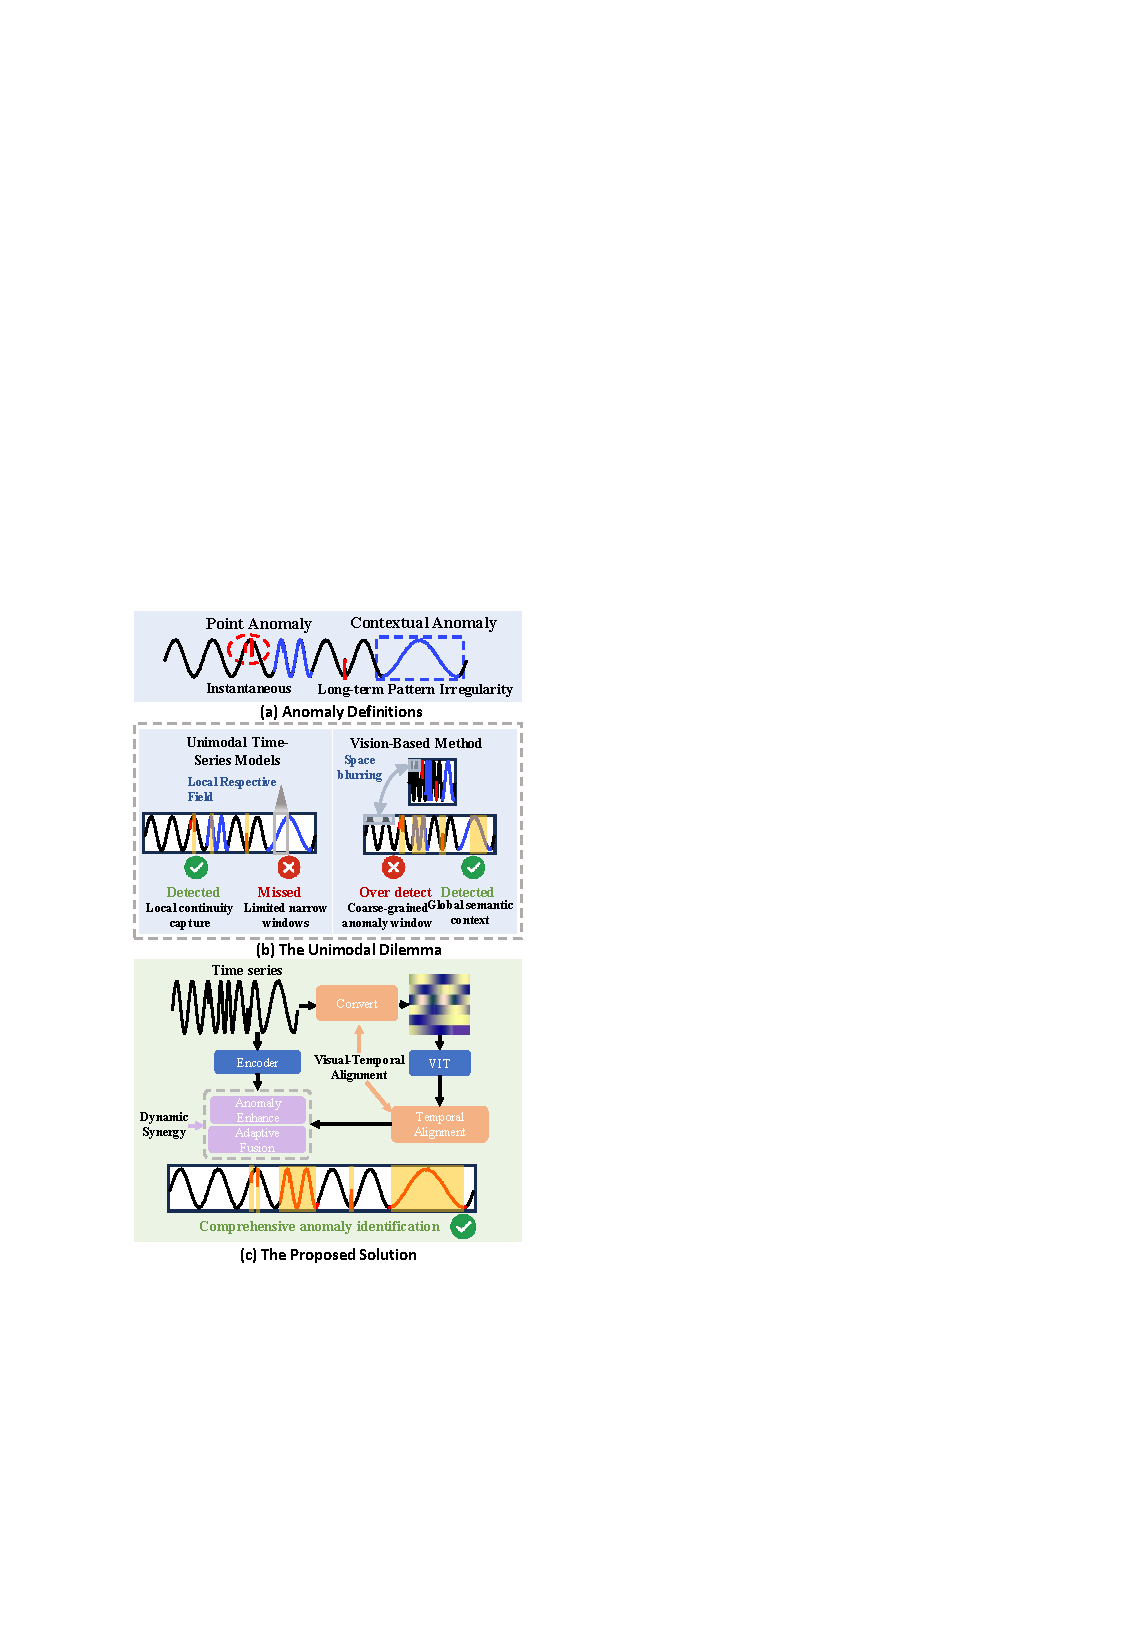
\includegraphics[width=0.9\linewidth]{IMG/img1.pdf}
    \caption{Comparison of the previous TSAD methods and the proposed VETime.}
    \label{fig:img1}
\vspace{-0.8em}
\end{figure}

To bridge these gaps, we propose VETime, the first framework that unifies temporal and visual features via effective alignment and fusion, enabling robust anomaly detection and precise localization, as shown in Figure \ref{fig:img1} (c).
To overcome the \textbf{alignment barrier}, we first develop a novel \textit{Reversible Image Conversion} method which constructs information-dense images with discriminative anomaly details.
Complementing this, we propose the \textit{Patch-Level Temporal Alignment} module, which enhances 2D visual representations from the pre-trained ViT with a 1D temporal ordering, establishing the structural basis for fine-grained cross-modal interaction. 
Subsequently, to facilitate \textbf{dynamic synergy}, we introduce two key mechanisms. Considering the distinct perceptual characteristics of visual and temporal modalities regarding anomalies, we propose a specialized \textit{Anomaly Window Contrastive Learning}. This incorporates intra- and inter-window Contrast between multi-modal features to achieve comprehensive anomaly identification. 
Finally, \textit{Task-Adaptive Multi-Modal Fusion} module equipped with a reconstruction head is applied to facilitate robust multi-modal fusion. This mechanism performs dynamic, adaptive weighted fusion of the aligned features, ensuring precise performance in downstream anomaly detection.
Our main contributions are listed as follows:
\begin{itemize}
    \item We propose VETime, the first TSAD framework that integrates visual and temporal features by fine-grained alignment and dynamic fusion, effectively exploiting the distinct perceptual advantages of each modality.

    \item We introduce an efficient Reversible Image Conversion module and a Patch-Level Temporal Alignment module, which jointly capture information-rich visual contexts while preserving critical temporal sensitivities.
    
    \item We introduce the Anomaly Window Contrastive Learning and Task-Adaptive Multi-Modal Fusion, synthesizing multi-modal complementary perceptual strengths to ensure comprehensive anomaly capture.

    \item Extensive experiments on multiple TSAD datasets prove that the proposed framework significantly outperforms existing SOTA models with lower computational costs compared to current vision-based methods.
\end{itemize}


\begin{figure*}[t]
    \centering
    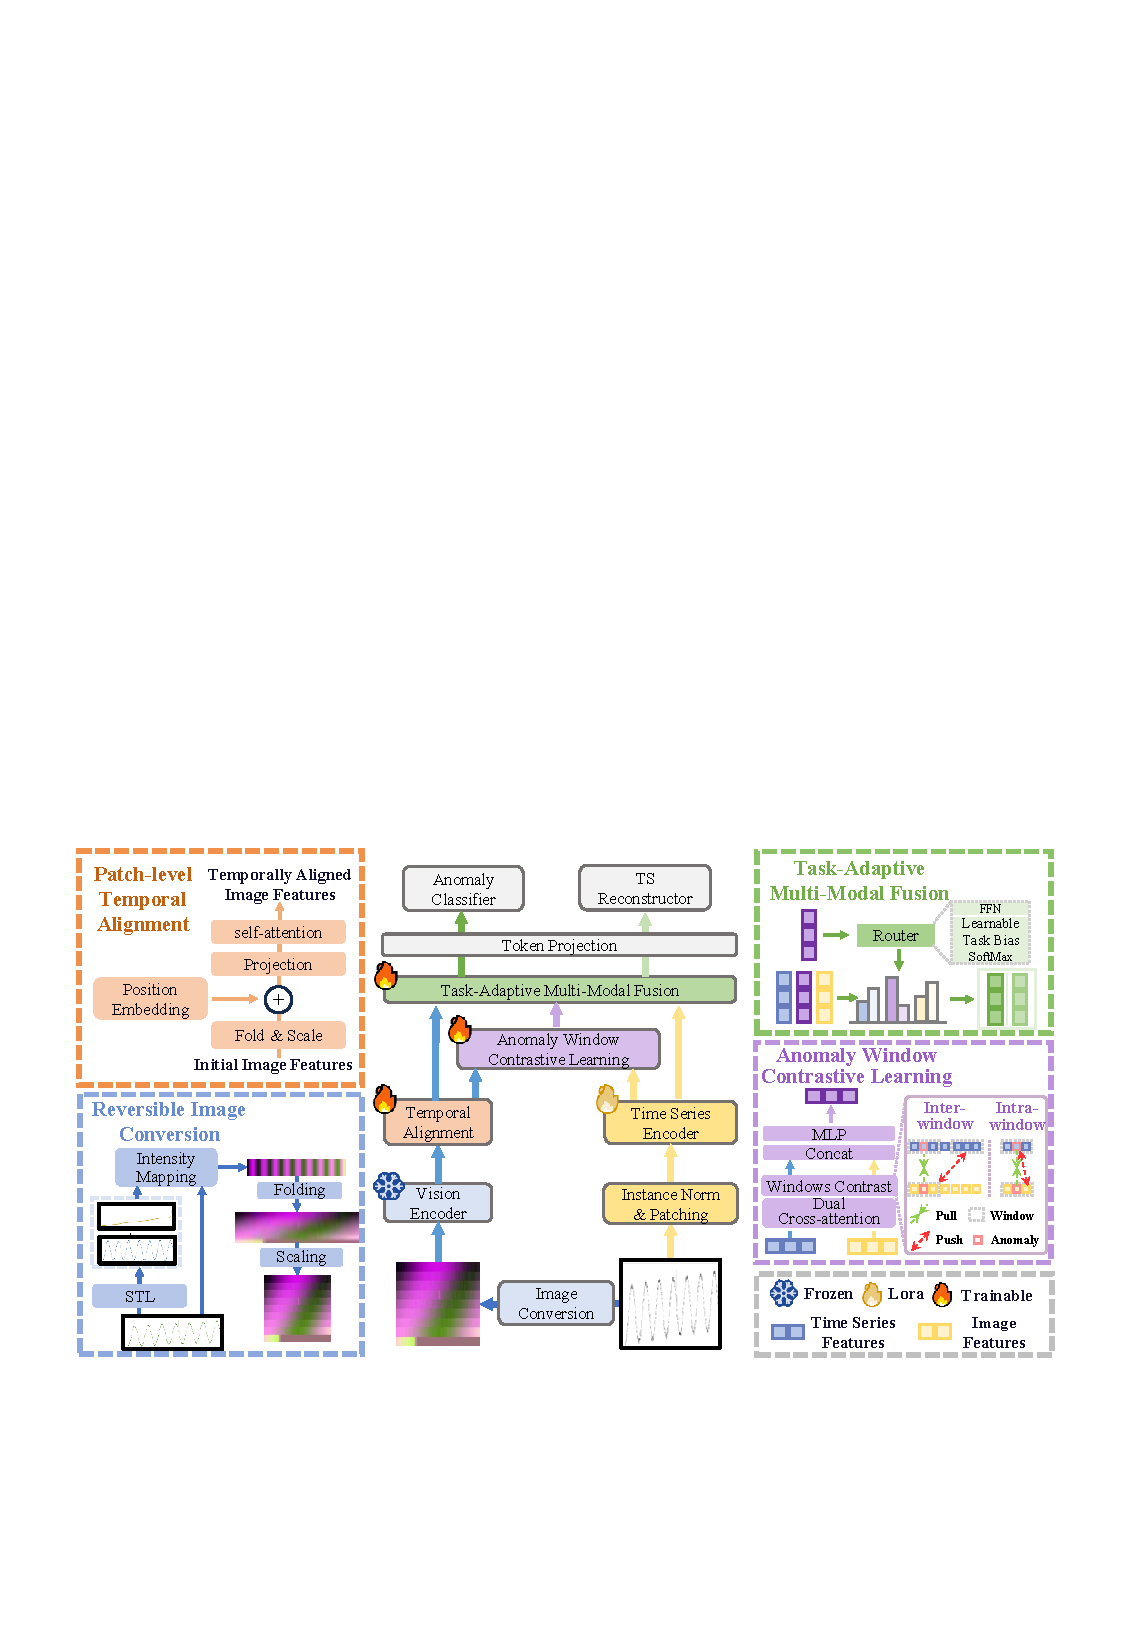
\includegraphics[width=0.9\linewidth]{IMG/img2.pdf}
    \caption{Overview of the proposed framework. The time series is first processed by a time-series encoder to extract temporal features $F_{TS}$ while simultaneously undergoing Reversible Image Conversion to generate visual input. Then visual features $F_{V_0}$ extracted from a frozen pre-trained image encoder are subsequently transformed into $F_V$ through Patch-Level Temporal Alignment to reinforce their temporal positional association. Then, $F_{TS}$ and $F_V$ are input into the Anomaly Window Contrastive Learning to derive an anomaly-enhanced representation $F_A$. Finally, a Task-Adaptive Multi-Modal Fusion module integrates all features ($F_A$, $F_{TS}$ , $F_V$). Final outputs $F_{AD}$ and $F_{Rec}$ are mapped to the original sequence length via token projection for the respective anomaly classification and reconstruction heads.}
    \label{fig:img2}
\end{figure*}
\vspace{-1em}
\section{Related Work} 

\subsection{Methods for TSAD} %malhotra2016lstm,,audibert2020usad,
Traditional TSAD algorithms primarily rely on reconstruction and forecasting paradigms~\cite{hundman2018detecting,su2019robust,tuli2022tranad}, they often struggle to generalize across diverse domains due to their training on specific datasets. To address these limitations, Time Series Foundation Models~\cite{shentu2024towards,goswami2024moment,ansari2024chronos,das2024decoder,lan2025foundationmodelszeroshottime} have emerged, attempting to capture universal patterns via large-scale pre-training.
% alongside LLMs~\cite{alnegheimish2024sigllm,zhou2024llmsunderstandtimeseries} that repurpose semantic engines for time-series analysis. 
However, TSFMs often suffer from over-generalization, where powerful reconstruction capabilities inadvertently reconstruct anomalies as well as normal data, masking the discrepancy required for detection.
A promising emerging direction involves visual approaches that leverage Vision-Language Models (VLMs) \cite{xu2025can,zhuang2024see,he2025harnessing} to capture global context under macroscopic perspective. 
Nevertheless, most existing works overlook the intrinsic perceptual complementarity between raw 1D temporal precision and 2D global visual context, falling short of effectively detecting both point and context anomalies in a unified framework.


\subsection{Vision-based Model for Time Series Analysis}

Vision-based time series analysis leverages computer vision backbones by transforming 1D temporal data into 2D representations ~\cite{ni2025harnessing}, mainly categorized into Line Plots~\cite{liu2024teaching,liu2024mllm4ts}, Heatmaps~\cite{chen2024visionts,wang2024timemixer}, and other transformation methods~\cite{yang2024vitime,ruan2024vision}. 
% To capture periodicity and multi-scale patterns, VisionTS~\cite{chen2024visionts} and TimeMixer++~\cite{wang2024timemixer} reshape signals into heatmaps or time-frequency scalograms, often framing forecasting as an image reconstruction task.
However, by treating the transformed visual representation as a holistic input, these pure vision-based approaches struggle to recover the precise sequential ordering of the original time series.
Recently, Time-VLM~\cite{zhong2025time} attempts to bridge this gap by mapping raw time-series features into the vision-language model (VLM) feature space for multimodal fusion. Nevertheless, it still fails to establish a strict alignment between the transformed image features and the original temporal axis, limiting its ability to support the precise localization of anomalies required for effective TSAD.

\begin{figure*}
    \centering
    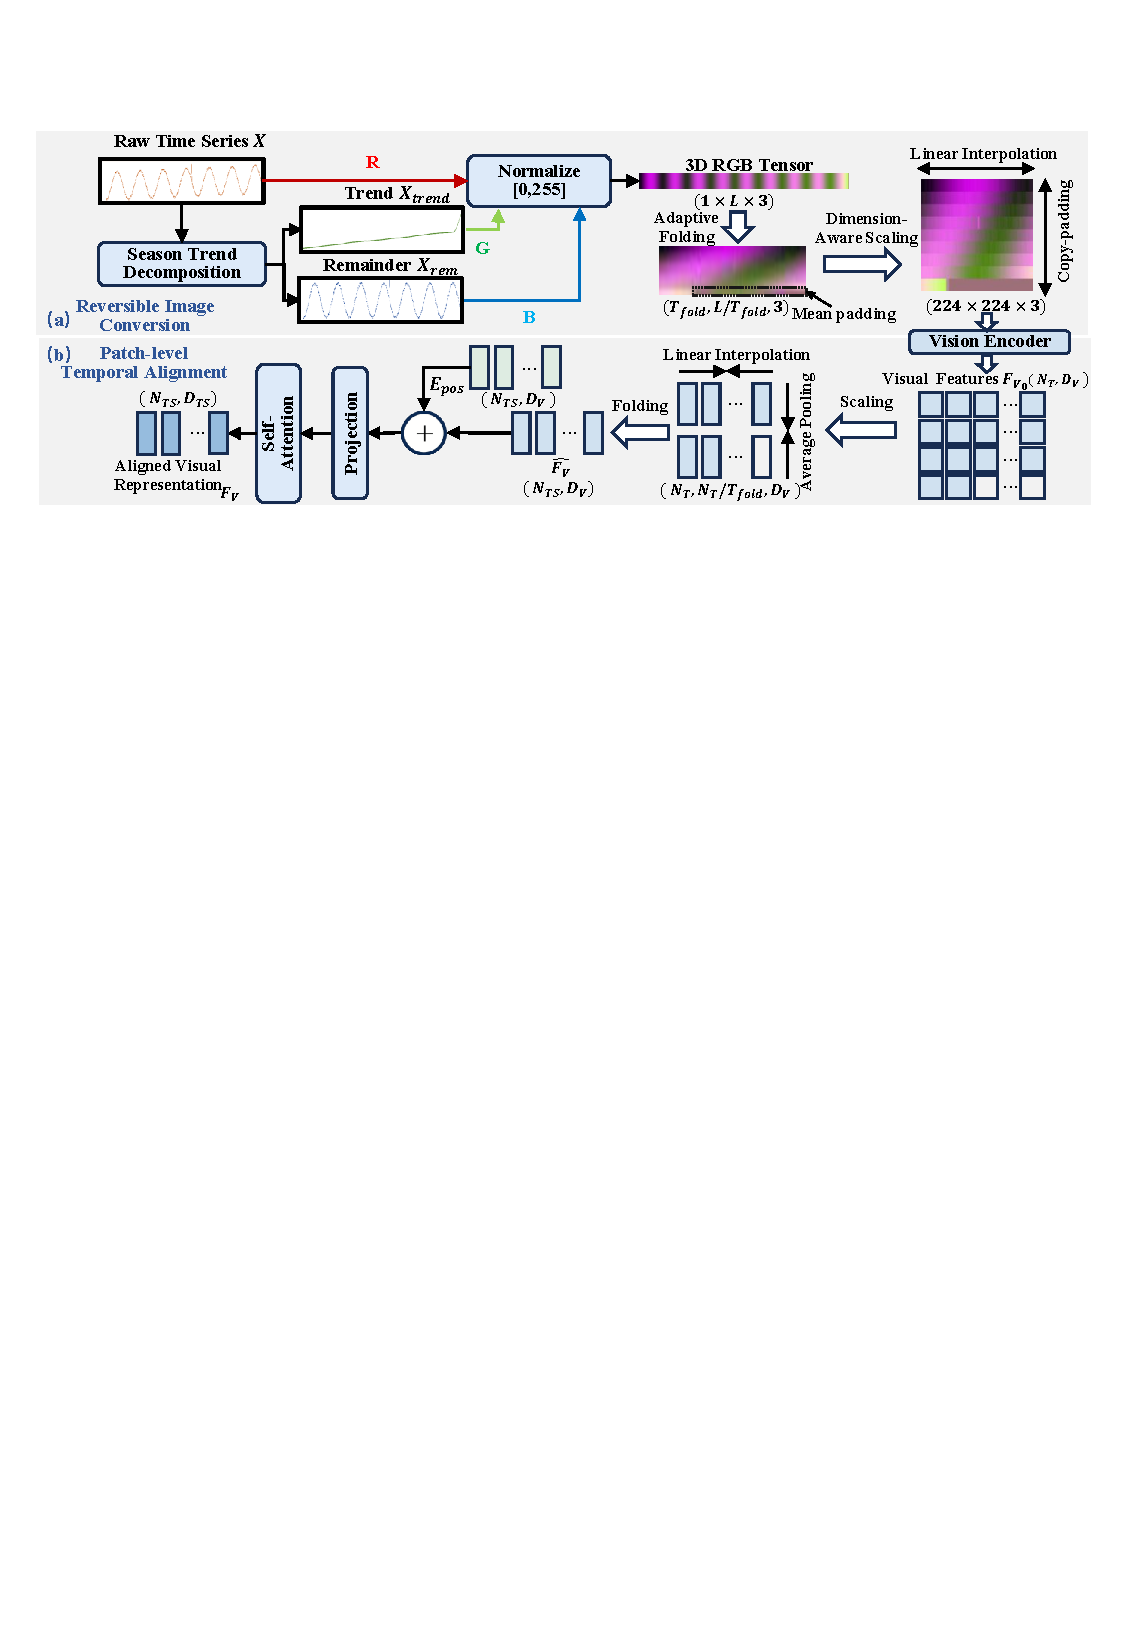
\includegraphics[width=0.9\linewidth]{IMG/img3.pdf}
    \caption{The framework of Reversible Image Conversion and Patch-level Temporal Alignment}
    \label{fig:img3}
\end{figure*}
\vspace{-1em}

\section{Methodology}

\subsection{Overview}
To harness the differentiated yet complementary advantages of temporal and visual modalities, we propose a unified framework capable of fine-grained temporal alignment and dynamic interaction for anomaly detection. As illustrated in Figure \ref{fig:img2}, the framework comprises four core components:

\begin{itemize}
    \vspace{-0.5em}
    \item \textbf{Reversible Image Conversion}: Transforms 1D time series into reversible visual representations. This module encapsulates both global and local correlations into semantically rich visual formats, thereby significantly accentuating anomalous patterns within the data.
    \vspace{-0.5em}
    \item \textbf{Patch-Level Temporal Alignment}: Realigns visual features to the temporal axis to ensure fine-grained semantic correspondence, establishing a robust prerequisite for the subsequent multi-scale interaction between global and local contexts.
    \vspace{-0.5em}
    \item \textbf{Anomaly Window Contrastive Learning}: 
    Leverages the complementary nature of visual and temporal modalities to enforce multi-scale discriminability for anomaly information. Through intra- and inter-window contrastive learning, this module facilitates the mutual reinforcement of visual and temporal features to effectively isolate anomaly patterns.
    \vspace{-0.5em}
    \item \textbf{Task-Adaptive Multi-Modal Fusion}: Dynamically integrates multimodal features to achieve end-to-end feature fusion. Specifically, it employs sequence reconstruction as an auxiliary constraint to promote deep feature interaction and comprehensive complementarity, ultimately generating robust anomaly representations. 
\end{itemize}
\vspace{-0.5em}
Ultimately, the fused representations capitalize on the synergy between temporal and visual domains, facilitating accurate localization across diverse anomaly types.
It is noted that our framework supports univariate and multivariate time series settings. The main text focuses on univariate cases, with the multivariate extension detailed in Appendix \ref{appendix:Multivariate}.


\subsection{Reversible Image Conversion:}
To accentuate the distinctiveness of anomalous signals while maintaining efficient information encoding, we transform univariate time series into high-density visual representations via a three-stage pipeline, as shown in Figure \ref{fig:img3} (a). 
\vspace{-0.5em}

\paragraph{Multi-Channel Intensity Mapping:}
Unlike prior single-channel mapping approaches \cite{chen2024visionts}, we employ a multi-channel encoding strategy, which capitalizes on the standard RGB architecture to incorporate denser information and better exposes latent anomalous patterns. Following DLinear \cite{Zeng2022AreTE}, the raw series $X \in \mathbb{R}^{L}$ is decomposed into a trend component $X_{trend}$ and a remainder component $X_{rem}$, where $L$ is the length of the series. The triplet $\{X, X_{trend}, X_{rem}\}$ is independently normalized to $[0, 255]$ and mapped to the R, G, and B channels, yielding a $1 \times L \times 3$ tensor that explicitly encompasses both global trends and high-frequency residuals.
\vspace{-0.5em}
\paragraph{Adaptive Folding:}
To accommodate diverse temporal scales, we adopt a periodicity-based folding strategy \cite{wu2023timesnet} to transform 1D sequence into a 2D grid with dimensions $(T_{fold}, \lceil L/T_{fold} \rceil, 3)$. The folding period $T_{fold}$ is dynamically estimated via the autocorrelation function (defaulting to $\sqrt{L}$ for non-periodic samples), and adjusted to be a multiple of the ViT patch size to prevent temporal information discontinuity. For indivisible lengths, we use the mean of the final period to pad trailing segments, minimizing distribution shifts compared to zero-padding.
\vspace{-0.5em}
\paragraph{Dimension-Aware Scaling:}
To standardize input resolution from $(T_{fold}, \lceil L/T_{fold} \rceil, 3)$ to $(224, 224, 3)$ without fidelity loss, we apply a decoupled scaling strategy. We use linear interpolation along the time axis (horizontal) to preserve waveform continuity, while employing a copy-padding strategy along the period axis (vertical) to prevent semantic distortion or pseudo-patterns that could arise from interpolation across distinct periods.

\vspace{-0.5em}
\subsection{Patch-Level Temporal Alignment}
The generated visual representations are fed into a frozen visual encoder to extract initial visual features $F_{V_0} \in \mathbb{R}^{N_V \times D_V}$. In parallel, the time series undergoes instance normalization and patching, followed by a temporal encoder to yield $F_{TS} \in \mathbb{R}^{N_{TS} \times D_{TS}}$. Here, $N$ and $D$ denote the patch count and feature dimension for the respective modalities. To bridge the structural discrepancy between modalities, we introduce a Patch-Level Temporal Alignment module for $F_{V_0}$ (Figure \ref{fig:img3} (b)).

Specifically, visual features are mapped back to the 1D temporal domain by inverting the folding logic. $F_{V_0}$ is reshaped to the initial 2D grid, linearly interpolated along the temporal axis to match the temporal patch count, and average-pooled along the periodicity axis to aggregate redundant repetitions. The resulting features are flattened to yield the concise aligned image features $\hat{F}_{V} \in \mathbb{R}^{N_{TS} \times D_V}$ .

Finally, to recover temporal context lost during visual encoding, we incorporate learnable positional encoding $E_{POS} \in \mathbb{R}^{N_{TS} \times D_V} $ followed by projection and self-attention layers to model intra- and inter-patch dependencies. Ultimately, this produces a visual representation $F_{V}$ that maintains temporal correspondence with $F_{TS}$.
% \chen{better mention time series instance norm, patching and encoder a bit as one short section, current have no idea what is $F_{TS}$, what is $N_{TS}$, $D_{TS}$}
\vspace{-0.5em}
\subsection{Anomaly Window Contrastive Learning}

Time-series and image features $F_{TS}$ and $F_{V}$ are first input into a dual cross-attention. Here, features from each modality serve as mutual queries to integrate complementary contexts, followed by a residual FFN for refinement, yielding updated representations $Z_{TS}$ and $Z_V$. The process is formulated as:
\begin{equation}
\begin{aligned}
    Z_{TS}^{0} &= \text{CrossAttn}(F_{TS}, F_V), \\
    Z_V^{0}    &= \text{CrossAttn}(F_V, F_{TS}), \\
    Z_{TS}       &= Z_{TS}^{0} + \text{FFN}\big(Z_{TS}^{0}\big),\\
    Z_V          &= Z_V^{0} + \text{FFN}\big(Z_V^{0}\big),
\end{aligned}
\end{equation}
where 
\begin{equation}
    \text{CrossAttn}(X, Y) = \text{Softmax}\left( \frac{X W_Q (Y W_K)^\top}{\sqrt{d}} \right) (Y W_V),
\end{equation}
denotes the cross-attention mechanism with $X$ serving as queries and $Y$ providing keys and values;  
$W_Q$, $W_K$, and $W_V \in \mathbb{R}^{d \times d}$ are learnable projection matrices;  
$d$ is the  dimension of the feature embeddings;  
and $\text{FFN}(\cdot)$ represents a feed-forward network applied with residual connection.

Given the inherent disparities between time-series and image features, specifically concerning their receptive fields and sensitivity to anomalies, we employ a hybrid strategy comprising Intra-Window and Inter-Window contrastive learning to explicitly model discriminative features across different scales, as shown in Figure \ref{fig:img4}.
\vspace{-0.5em}
\paragraph{Anomaly Context Windows:}
To facilitate this, we construct adaptive windows around anomalies. Point-level labels are converted to binary patch-level labels (set to 1 if any timestamp within the patch is anomalous). Then, for a continuous anomaly segment spanning $L_a$ patches, we define an Anomaly Context Window by symmetrically extending the normal segment on both sides, with a maximum length of $L_w = 2 L_a$. Each window contains one continuous anomaly instance surrounded by its immediate local context.
\vspace{-0.5em}
\paragraph{Intra-Window Contrastive Learning:}
Designed to capture short-duration point anomalies ($L_w \le 1$ patches, like outliers), this component enforces fine-grained anomaly alignment for visual feature  $Z_{V}$. Within a window, the visual feature at the anomaly position serves as the anchor $Z_{V}^{A}$, paired with the corresponding temporal feature as the positive sample $Z_{TS}^{A}$. Normal temporal features within the same window act as negatives $Z_{TS}^{N}$. The intra-window contrastive loss $\mathcal{L}_{intra}$ is defined as:
\begin{equation}
\mathcal{L}_{intra} = - \log \frac{\exp(Z_{V}^{A} \cdot Z_{TS}^{A})/\tau)}{\sum_{k \in \mathcal{N}_{neg}} \exp(Z_{V}^{A}\cdot Z_{TS}^{k})/\tau)},
\end{equation}
where $\cdot$ denotes dot product similarity, $\tau$ is the temperature parameter, and $\mathcal{N}_{neg}$ represents the set of normal features within the window.
\vspace{-0.5em}
\paragraph{Inter-Window Contrastive Learning:}
For long-duration context anomalies ($L_w \ge$ 2  patches, like seasonal anomaly), we enhance global discriminability for temporal feature  $Z_{TS}$. We aggregate features along the temporal dimension within each window using average pooling. The pooled time-series feature of an anomaly window $\bar{Z}_{TS}^{A}$ serves as the anchor, paired with its visual counterpart $\bar{Z}_{V}^{A}$, while pooled features from normal windows $\bar{Z}_{V}^{N}$ serve as negatives.The inter-window contrastive loss $\mathcal{L}_{inter}$ is:

\begin{equation}
\mathcal{L}_{inter} = - \log \frac{\exp(\bar{Z}_{TS}^{A}\cdot \bar{Z}_{V}^{A})/\tau)}{\sum_{j \in \mathcal{W}_{neg}} \exp(\bar{Z}_{TS}^{A}\cdot \bar{Z}_{V}^{j})/\tau)}
\end{equation}
where $\mathcal{W}_{neg}$ denotes the set of normal window features.

\paragraph{Total contrastive Loss:} The total contrastive loss $\mathcal{L}_{aw}$ is:
\begin{equation}
\mathcal{L}_{aw} = \frac{1}{N} \sum_{i=1}^{N} ( \frac{1}{W_s}\sum_{s=1}^{W_s} \mathcal{L}_{intra}^{(s)} +\frac{1}{W_l}\sum_{l=1}^{W_l} \mathcal{L}_{inter}^{(l)}), 
\end{equation}
where $N$ is the number of samples, $W_s$ and $W_l$ are the number of short and long anomalies in each instance, respectively. Crucially, this loss is calculated independently for each sample. This design choice avoids interference caused by the distinct variability of normal and anomalous patterns across different instances, ensuring robust feature learning. 

Finally, the enhanced features are concatenated and processed by a Feed-Forward Network (FFN) to yield the anomaly representation $F_A= {\text{FFN}}([Z_{TS};Z_{V}])$, where $[\cdot;\cdot]$ denotes feature concatenation.


\begin{figure}
    \centering
    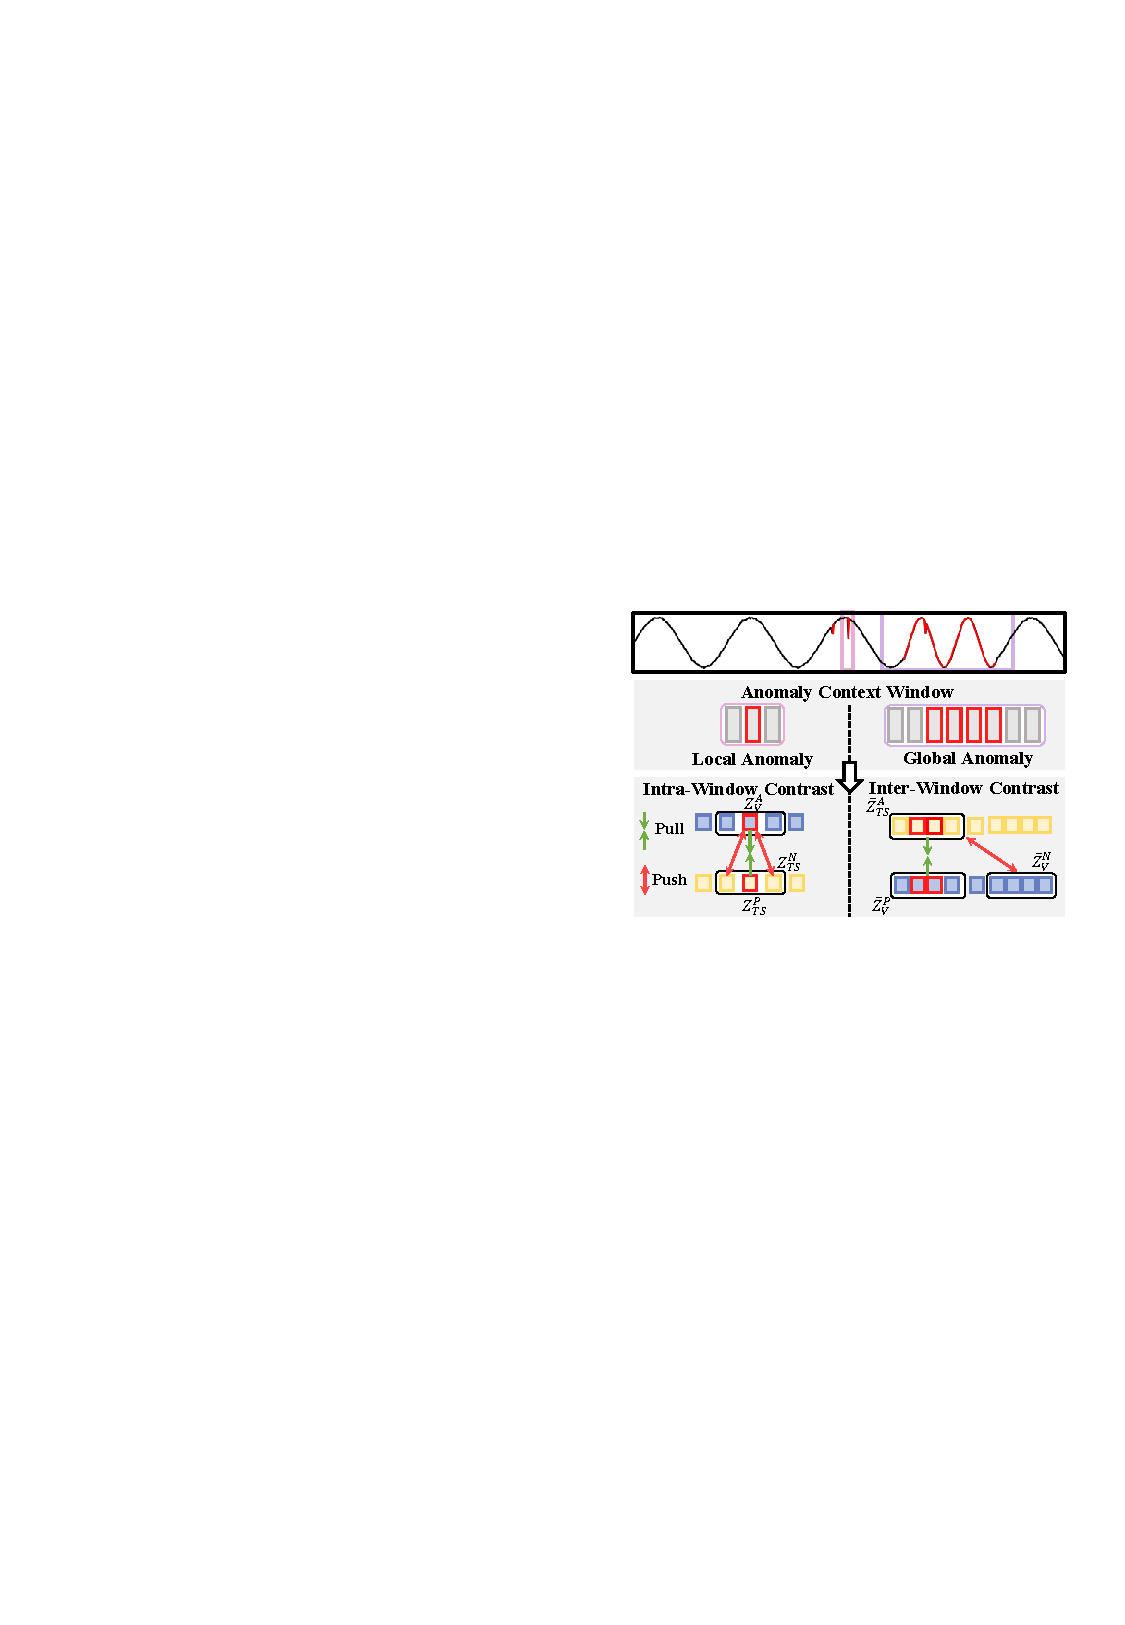
\includegraphics[width=0.8\linewidth]{IMG/img4.pdf}
    \caption{An illustration of Anomaly Window Contrastive Learning}
    \label{fig:img4}
\end{figure}
\vspace{-0.9em}

\subsection{Task-Adaptive Multi-Modal Fusion}
To realize dynamic semantic integration and efficient end-to-end training, we propose a Task-Adaptive Multi-modal Fusion Module. This module acts as a dynamic routing mechanism, treating time-series ($F_{TS}$), vision ($F_{V}$), and anomaly-enhanced ($F_{A}$) features as  experts in a candidate space.
\vspace{-0.5em}
\paragraph{Dynamic Weight Routing:}
A routing network computes patch-level dynamic weights $w \in \mathbb{R}^{N_{TS} \times 3 \times 2}$ to assign importance to each expert for the two downstream tasks (anomaly detection and reconstruction). Specifically, weights are generated via a learnable task-specific bias $\mathbf{b}_{task}\in\mathbb{R}^{N_{TS} \times D_{TS} \times 2}$ added:

\begin{equation}
w = \text{Softmax}(\text{MLP}(F_A) + \mathbf{b}_{task})
\end{equation}

where the Softmax is applied across the expert dimension. 

To prevent expert collapse where the router relies solely on a single modality, we impose an entropy-based regularization to encourage diverse expert utilization:
\begin{equation}
\mathcal{L}_e = \frac{1}{2N_{TS}} \sum_{i=1}^{N_{TS}} \sum_{t=1}^{2} \sum_{m \in \{TS, V, A\}} w_{i,m,t} \log w_{i,m,t}
\end{equation}
where $N_{TS}$ denotes the number of temporal patches, $t \in \{1, 2\}$ indexes the two downstream tasks including anomaly detection and reconstruction, $m$ iterates over the three features, and $w_{i,m,t}$ represents the dynamic fusion weight assigned to modality $m$ for patch $i$ in task $t$.

\paragraph{Task-Adaptive Fusion:}
The final fused $F_{Fused}$ is obtained by the weighted summation of the expert features:
\begin{equation}
F_{Fused} = \sum_{m \in \{TS, V, A\}} w_{m} \cdot F_{m} 
\end{equation}
where $F_{Fused}=[F_{AD},F_{Rec}]$ is subsequently used for anomaly detection and reconstruction tasks. Crucially, we employ sequence reconstruction as an auxiliary task rather than a primary objective. By requiring the fused features to reconstruct the original input, we encourage the preservation of rich semantic content and foster deep multimodal interaction. This auxiliary constraint prevents the model from overfitting to sparse anomaly labels, ultimately yielding a more robust representation for the primary anomaly detection task.


\subsection{Optimization}
The features $F_{AD}$ and $F_{Rec}$ are projected to the original sequence length and fed into separate specific heads. The model is trained via a multi-task objective:
\begin{equation}
\mathcal{L}_{total} = \mathcal{L}_{BCE} + \mathcal{L}_{MSE} + \lambda_{aw} \mathcal{L}_{aw} + \lambda_{e} \mathcal{L}_{e}
\end{equation}
where $\mathcal{L}_{BCE}$ and $\mathcal{L}_{MSE}$ target anomaly classification and sequence reconstruction, the detailed computation is provided in Appendix \ref{appx.loss}. $\lambda$ is the weights of different $\mathcal{L}$.


\begin{table*}[t!]
    \centering
    \renewcommand{\arraystretch}{0.75}
    \caption{
        Performance of VETime against zero-shot and full-shot baselines in 11 public univariate datasets. The models marked with (\(\dagger\)) were excluded where necessary due to potential data leakage under zero-shot setting. Asterisked (*) results are excluded from ranking due to data leaking. \textcolor{red}{Red}: best,\textcolor{blue}{Blue}: second best.
    }
    \label{tab:tab1}
    \resizebox{\textwidth}{!}{%
    \begin{tabular}
    % {l|l|ccccccccccc|c|c|c}
    {
    >{\centering\arraybackslash}p{1.8cm}
    |>{\centering\arraybackslash}p{2.0cm}
    |*{11}{>{\centering\arraybackslash}p{1.1cm}|}
    *{3}{>{\centering\arraybackslash}p{0.55cm}}
    }
    
        \hline
        \multirow{2}{*}{\textbf{Metric}} & \multirow{2}{*}{\textbf{Model}} & \multicolumn{11}{c|}{\textbf{Univariate Datasets}} & \textbf{Total} & \textbf{Total}& \textbf{Avg} \\
        \cline{3-13}
        & & \textbf{IOPS} & \textbf{MGAB} & \textbf{NAB} & \textbf{NEK} & \textbf{Power} & \textbf{SED} & \textbf{Stock} & \textbf{TODS} & \textbf{UCR} & \textbf{WSD} & \textbf{YAHOO} & \textbf{1st} & \textbf{2nd}& \textbf{Rank} \\
        \hline
        \multicolumn{16}{c}{\textbf{Zero-Shot Models}} \\
        \hline
        \multirow{8}{*}{Affiliation-F1} & VETime      & \textcolor{red}{\textbf{90.53}} & \textcolor{blue}{\textbf{68.03}} & \textcolor{blue}{\textbf{88.57}} & 79.56 & \textcolor{blue}{\textbf{78.78}} & \textcolor{red}{\textbf{97.31}} & 69.60 & 85.85 & \textcolor{red}{\textbf{85.06}} & \textcolor{blue}{\textbf{94.31}} & \textcolor{red}{\textbf{97.15}} & \textcolor{red}{\textbf{04}}& \textcolor{red}{\textbf{04}} &\textcolor{red}{\textbf{2.55}}\\
        & TimeRCD     & 83.28 & \textcolor{red}{\textbf{70.69}} & 82.48 & 79.73 & \textcolor{red}{\textbf{85.51}} & \textcolor{blue}{\textbf{96.87}} & 71.84 & 86.37 & \textcolor{blue}{\textbf{84.63}} & 90.33 & \textcolor{blue}{\textbf{96.65}} & \textcolor{blue}{\textbf{02}} & \textcolor{blue}{\textbf{03}}&\textcolor{blue}{\textbf{3.27}}\\
        & DADA†   & 89.37\rlap{*} & 67.66\rlap{*} & 86.56 & \textcolor{red}{\textbf{95.40}} & 69.79 & 65.18 & \textcolor{red}{\textbf{98.77}} & 76.89 & 72.21 & 93.92 & 92.20\rlap{*} & \textcolor{blue}{\textbf{02}} & 00&4.00 \\
        & TS-Pulse    & 68.76 & 67.33 & 70.80 & 73.05 & 69.94 & 67.44 & 67.93 & 67.90 & 67.70 & 68.22 & 70.05 & 00 & 00 &6.64\\
        & MOMENT†     & 87.54\rlap{*} & 66.76\rlap{*} & \textcolor{red}{\textbf{90.45}}\rlap{*} & 92.26 & 75.97 & 59.13 & 45.26 & 59.76 & 75.77 & \textcolor{red}{\textbf{95.39}} & 79.99\rlap{*} & \textcolor{blue}{\textbf{02}} & 00 &4.73\\
        & TimesFM     & 81.88 & 66.95 & 79.73 & 90.49 & 69.88 & 67.14 & \textcolor{blue}{\textbf{97.53}} & \textcolor{blue}{\textbf{89.08}} & 70.03 & 78.97 & 91.28 & 00 & 02&5.27 \\
        & Chronos     & \textcolor{blue}{\textbf{90.12}} & 67.89 & 86.66 & \textcolor{blue}{\textbf{93.63}} & 69.72 & 67.89 & 96.85 & \textcolor{red}{\textbf{91.96}} & 74.35 & 90.98 & 96.34 & 01 & 02 &\textcolor{blue}{\textbf{3.27}}\\
        & Time MOE    & 76.34 & 67.23 & 80.51 & 80.50 & 71.19 & 60.98 & 63.28 & 54.68 & 73.56 & 80.25 & 69.70 & 00 & 00&6.27 \\
        \hline
        \multirow{8}{*}{F1\_T} & VETime & \textcolor{blue}{\textbf{46.15}} & \textcolor{red}{\textbf{2.00}} & \textcolor{red}{\textbf{44.31}} & \textcolor{blue}{\textbf{60.86}} & \textcolor{blue}{\textbf{20.16}} & \textcolor{red}{\textbf{74.35}} & 22.41 & \textcolor{red}{\textbf{68.33}} & \textcolor{red}{\textbf{36.25}} & \textcolor{red}{\textbf{50.42}} & \textcolor{red}{\textbf{91.54}} & \textcolor{red}{\textbf{07}} & \textcolor{blue}{\textbf{03}} &\textcolor{red}{\textbf{1.91}}\\
        & TimeRCD & 28.44 & \textcolor{blue}{\textbf{01.81}} & \textcolor{blue}{\textbf{38.85}} & 35.87 & \textcolor{red}{\textbf{28.47}} & \textcolor{blue}{\textbf{69.43}} & 31.73 & \textcolor{blue}{\textbf{65.89}} & \textcolor{blue}{\textbf{34.30}} & 35.04 & \textcolor{blue}{\textbf{85.86}} & \textcolor{blue}{\textbf{01}} & \textcolor{red}{\textbf{06}} &\textcolor{blue}{\textbf{3.27}}\\
        & DADA† & 42.50\rlap{*} & 00.91\rlap{*} & 37.24 & 47.98 & 19.80 & 09.56 & \textcolor{red}{\textbf{95.49}} & 35.18 & 07.22 & \textcolor{blue}{\textbf{48.46}} & 79.52\rlap{*} & \textcolor{blue}{\textbf{01}} & 05 &4.45\\
        & TS-Pulse & 04.10 & 00.81 & 34.61 & 27.07 & 19.90 & 09.71 & 15.98 & 13.45 & 05.12 & 4.57 & 05.50 & \textcolor{blue}{\textbf{01}} & 01 &7.00\\
        & MOMENT† & 33.15\rlap{*} & 00.80\rlap{*} & 52.27\rlap{*} & \textcolor{red}{\textbf{63.66}} & 19.91 & 09.54 & 18.04 & 17.47 & 13.02 & 41.98 & 11.69\rlap{*} & \textcolor{blue}{\textbf{01}} & 00&5.00 \\
        & TimesFM & \textcolor{red}{\textbf{48.95}} & 00.93 & 36.74 & 36.63 & 19.80 & 09.58 & \textcolor{blue}{\textbf{88.94}} & 51.13 & 41.38 & 10.78 & 83.46 & \textcolor{blue}{\textbf{01}} & 01&4.18 \\
        & Chronos & 45.45 & 01.10 & 36.10 & 33.16 & 19.90 & 13.18 & 89.3 & 53.90 & 10.88 & 39.82 & 79.00 & 00 & 00 &4.27\\
        & Time MOE & 25.95 & 00.63 & 38.70 & 15.78 & 19.85 & 17.73 & 34.13 & 20.91 & 08.29 & 22.6 & 37.11 & 00 & 00&5.91 \\
        \hline
        \multirow{8}{*}{Standard-F1} & VETime & \textcolor{red}{\textbf{34.56}} & \textcolor{red}{\textbf{1.89}} & \textcolor{red}{\textbf{37.87}} & \textcolor{blue}{\textbf{53.95}} & \textcolor{blue}{\textbf{20.12}} & \textcolor{red}{\textbf{75.02}} & 23.83 & \textcolor{red}{\textbf{69.13}} & \textcolor{red}{\textbf{30.61}} & \textcolor{red}{\textbf{46.55}} & \textcolor{red}{\textbf{88.93}} & \textcolor{red}{\textbf{08}} & \textcolor{blue}{\textbf{02}}&\textcolor{red}{\textbf{1.73}} \\
        & TimeRCD & 24.22 & \textcolor{blue}{\textbf{01.62}} & \textcolor{blue}{\textbf{27.70}} & 33.05 & \textcolor{red}{\textbf{28.59}} & \textcolor{blue}{\textbf{69.88}} & 32.61 & \textcolor{blue}{\textbf{67.02}} & \textcolor{blue}{\textbf{28.13}} & 31.96 & \textcolor{blue}{\textbf{87.02}} & \textcolor{blue}{\textbf{01}} & \textcolor{red}{\textbf{06}} &\textcolor{blue}{\textbf{3.27}}\\
        & DADA† & 32.76\rlap{*} & 00.80\rlap{*} & 26.91 & 48.24 & 15.99 & 02.69 & \textcolor{red}{\textbf{95.59}} & 28.18 & 03.36 & \textcolor{blue}{\textbf{45.06}} & 79.30\rlap{*} & \textcolor{blue}{\textbf{01}} & 05&4.36 \\
        & TS-Pulse & 03.54 & 00.73 & 21.61 & 23.96 & 18.27 & 08.84 & 15.46 & 12.45 & 02.05 & 2.17 & 04.00 & 00 & 00 &6.82\\
        & MOMENT† & 30.69\rlap{*} & 00.67\rlap{*} & 44.75\rlap{*} & \textcolor{red}{\textbf{63.85}} & 16.39 & 03.36 & 19.38 & 14.64 & 09.00 & 41.42 & 10.54\rlap{*} & \textcolor{blue}{\textbf{01}} & 00&4.73 \\
        & TimesFM & \textcolor{blue}{\textbf{34.28}} & 00.83 & 26.46 & 38.15 & 16.73 & 02.96 & 89.13 & 40.08 & 07.86 & 38.5 & 84.44 & \textcolor{blue}{\textbf{01}} & 01 &4.27\\
        & Chronos & 32.69 & 00.99 & 26.22 & 33.54 & 17.47 & 08.74 & \textcolor{blue}{\textbf{89.41}} & 40.52 & 08.21 & 34.58 & 78.89 & 00 & 00 &4.55\\
        & Time MOE & 26.52 & 00.45 & 26.20 & 11.47 & 12.16 & 17.73 & 34.32 & 16.38 & 04.09 & 20.09 & 27.50 & 00 & 00 &6.55\\
        \hline
        \multirow{8}{*}{VUS-PR} & VETime & \textcolor{red}{\textbf{30.79}} & \textcolor{blue}{\textbf{0.70}}& \textcolor{red}{\textbf{32.98}} & \textcolor{blue}{\textbf{57.54}} & \textcolor{blue}{\textbf{11.78}} & \textcolor{red}{\textbf{89.05}} & 76.08 & \textcolor{red}{\textbf{94.20}} & \textcolor{red}{\textbf{24.99}} & \textcolor{blue}{\textbf{33.85}} & \textcolor{red}{\textbf{88.61}} & \textcolor{red}{\textbf{06}} & \textcolor{red}{\textbf{04}}&\textcolor{red}{\textbf{2.00}} \\
        & TimeRCD & \textcolor{blue}{\textbf{20.23}} & \textcolor{red}{\textbf{01.05}} & 24.32 & 27.88 & \textcolor{red}{\textbf{21.25}} & \textcolor{blue}{\textbf{80.75}} & 77.28 & \textcolor{blue}{\textbf{93.46}} & \textcolor{blue}{\textbf{23.09}} & 21.77 & 84.41 & \textcolor{blue}{\textbf{02}} & \textcolor{red}{\textbf{04}}&\textcolor{blue}{\textbf{3.09}} \\
        & DADA† & 24.97\rlap{*} & 00.57\rlap{*} & \textcolor{blue}{\textbf{24.73}} & 46.85 & 10.61 & 06.42 & \textcolor{red}{\textbf{99.51}} & 64.83 & 02.94 & 33.42 & 70.74\rlap{*} & 01 & 01 &4.00\\
        & TS-Pulse & 04.64 & 00.56 & 16.40 & 19.39 & 11.72 & 09.11 & 70.95 & 45.86 & 01.20 & 1.83 & 09.93 & 00 & 00&6.82 \\
        & MOMENT† & 37.35\rlap{*} & 00.56\rlap{*} & 45.38\rlap{*} & \textcolor{red}{\textbf{67.74}} & 10.50 & 04.31 & 76.97 & 56.45 & 06.17 & \textcolor{red}{\textbf{55.26}} & 30.81\rlap{*} & \textcolor{blue}{\textbf{02}} & 00&3.73 \\
        & TimesFM & 19.56 & 00.58 & 24.01 & 35.02 & 10.44 & 06.13 & \textcolor{blue}{\textbf{98.39}} & 72.89 & 06.03 & 21.57 & \textcolor{blue}{\textbf{86.78}} & 00 & \textcolor{blue}{\textbf{02}} &4.45\\
        & Chronos & 19.00 & 00.60 & 23.76 & 31.80 & 10.95 & 08.65 & 97.49 & 70.66 & 06.56 & 18.81 & 83.54 & 00 & 00&4.91 \\
        & Time MOE & 16.63 & 00.52 & 22.62 & 19.76 & 09.34 & 10.87 & 74.78 & 48.78 & 02.10 & 10.93 & 20.90 & 00 & 00&6.82 \\
        \hline
        \multicolumn{13}{l}{\textbf{\ Grand Total (Zero-Shot)}} & \textbf{25} & \textbf{13} & \textbf{2.05}\\
        \hline
        \multicolumn{15}{c}{\textbf{Full-Shot Models}} \\
        \hline
        \multirow{6}{*}{Affiliation-F1} & VETime & \textcolor{red}{\textbf{90.53}} & 68.03 & 88.57 & 79.56 & \textcolor{red}{\textbf{78.78}} & \textcolor{red}{\textbf{97.31}} & 69.60 & \textcolor{red}{\textbf{85.85}} & \textcolor{red}{\textbf{85.06}} & \textcolor{red}{\textbf{94.31}} & \textcolor{red}{\textbf{97.15}} & \textcolor{red}{\textbf{07}} & 00 &\textcolor{red}{\textbf{1.91}}\\
        & TranAD & \textcolor{blue}{\textbf{83.19}} & 67.28 & 90.28 & \textcolor{blue}{\textbf{85.02}} & 71.56 & 61.03 & 57.94 & 52.76 & 73.31 & \textcolor{blue}{\textbf{84.34}} & \textcolor{blue}{\textbf{76.08}} & 00 & \textcolor{red}{\textbf{04}}&3.45 \\
        & USAD & 71.08 & 67.81 & \textcolor{blue}{\textbf{91.54}} & 71.13 & 76.48 & 55.60 & 35.92 & 47.90 & \textcolor{blue}{\textbf{76.00}} & 65.10 & 53.05 & 00 & \textcolor{blue}{\textbf{02}}&4.36 \\
        & OmniAnomaly & 80.32 & 67.35 & \textcolor{red}{\textbf{92.35}} & \textcolor{red}{\textbf{86.30}} & \textcolor{blue}{\textbf{78.16}} & 61.26 & \textcolor{red}{\textbf{75.24}} & 50.73 & 73.53 & 78.02 & 71.31 & \textcolor{blue}{\textbf{03}} & 01&\textcolor{blue}{\textbf{3.00}} \\
        & LOF & 81.06 & \textcolor{blue}{\textbf{68.44}} & 75.75 & 84.74 & 66.76 & \textcolor{blue}{\textbf{63.85}} & \textcolor{blue}{\textbf{69.74}} & \textcolor{blue}{\textbf{60.58}} & 73.53 & 81.29 & 75.63 & 00 & \textcolor{red}{\textbf{04}} &3.09\\
        & IForest & 52.81 & \textcolor{red}{\textbf{68.82}} & 39.84 & 71.15 & 00.00 & 70.09 & 0.06 & 44.17 & 50.56 & 41.24 & 33.30 & 01 & 00&5.09 \\
        \hline
        \multirow{6}{*}{F1\_T} & VETime & \textcolor{blue}{\textbf{46.15}} & \textcolor{blue}{\textbf{2.00}} & \textcolor{blue}{\textbf{44.31}} & 60.86 & 20.16 & \textcolor{red}{\textbf{74.35}} & 22.41 & \textcolor{red}{\textbf{68.33}} & \textcolor{red}{\textbf{36.25}} & \textcolor{red}{\textbf{50.42}} & \textcolor{red}{\textbf{91.54}} & \textcolor{red}{\textbf{05}} & \textcolor{blue}{\textbf{03}} &\textcolor{red}{\textbf{2.09}}\\
        & TranAD & 22.63 & 01.65 & 37.28 & 69.97 & 22.36 & 09.57 & 16.73 & 13.51 & 07.75 & 20.94 & 08.41 & 00 & 00 &4.18\\
        & USAD & 20.99 & \textcolor{red}{\textbf{04.07}} & \textcolor{red}{\textbf{61.46}} & \textcolor{blue}{\textbf{70.64}} & \textcolor{red}{\textbf{28.23}} & 09.54 & 16.86 & 20.85 & \textcolor{blue}{\textbf{14.63}} & 14.18 & 09.35 & \textcolor{blue}{\textbf{03}} & 02 &3.18\\
        & OmniAnomaly & \textcolor{red}{\textbf{51.17}} & 01.61 & 40.09 & \textcolor{red}{\textbf{82.20}} & \textcolor{blue}{\textbf{23.48}} & \textcolor{blue}{\textbf{09.68}} & \textcolor{blue}{\textbf{36.22}} & 14.33 & 08.47 & \textcolor{blue}{\textbf{34.79}} & 24.16 & 02 & \textcolor{red}{\textbf{04}}&\textcolor{blue}{\textbf{3.09}} \\
        & LOF & 27.97 & 01.15 & 35.76 & 63.57 & 19.80 & 09.60 & \textcolor{red}{\textbf{66.14}} & \textcolor{blue}{\textbf{31.63}} & 08.31 & 24.38 & \textcolor{blue}{\textbf{55.93}} & 01 & 02&3.45 \\
        & IForest & 07.64 & 00.84 & 21.44 & 65.56 & 00.00 & 09.54 & 1.10 & 11.06 & 06.36 & 4.28 & 04.90 & 00 & 00 &5.00\\
        \hline
        \multirow{6}{*}{Standard-F1} & VETime & 34.56 & \textcolor{blue}{\textbf{1.89}} & \textcolor{blue}{\textbf{37.87}} & 53.95 & 20.12 & \textcolor{red}{\textbf{75.02}} & 23.83 & \textcolor{red}{\textbf{69.13}} & \textcolor{red}{\textbf{30.61}} & \textcolor{red}{\textbf{56.55}} & \textcolor{red}{\textbf{88.93}} & \textcolor{red}{\textbf{05}} & \textcolor{blue}{\textbf{02}}&\textcolor{red}{\textbf{2.00}} \\
        & TranAD & \textcolor{blue}{\textbf{34.85}} & 01.46 & 27.33 & 60.36 & 22.36 & 02.63 & 16.23 & 11.94 & 04.40 & 20.23 & 05.70 & 00 & 01 &3.91\\
        & USAD & 30.66 & \textcolor{red}{\textbf{03.89}} & \textcolor{red}{\textbf{56.15}} & \textcolor{blue}{\textbf{62.91}} & \textcolor{red}{\textbf{28.24}} & 03.41 & 17.99 & 23.87 & \textcolor{blue}{\textbf{10.74}} & 13.20 & 07.21 & \textcolor{blue}{\textbf{03}} & \textcolor{blue}{\textbf{02}}&\textcolor{blue}{\textbf{2.73}} \\
        & OmniAnomaly & \textcolor{red}{\textbf{47.05}} & 01.44 & 28.81 & \textcolor{red}{\textbf{74.03}} & \textcolor{blue}{\textbf{23.50}} & 00.43 & \textcolor{blue}{\textbf{38.59}} & 12.65 & 05.11 & \textcolor{blue}{\textbf{29.57}} & 21.40 & 02 & \textcolor{red}{\textbf{03}} &3.36\\
        & LOF & 30.28 & 01.05 & 24.04 & 56.92 & 12.18 & \textcolor{blue}{\textbf{04.11}} & \textcolor{red}{\textbf{66.20}} & \textcolor{blue}{\textbf{25.77}} & 04.70 & 22.62 & \textcolor{blue}{\textbf{48.95}} & 01 & \textcolor{red}{\textbf{03}}&3.55\\
        & IForest & 08.37 & 00.73 & 29.41 & 58.10 & 19.77 & 03.81 & 16.91 & 13.35 & 04.09 & 2.07 & 03.20 & 00 & 00 &5.09\\
        \hline
        \multirow{6}{*}{VUS-PR} & VETime & \textcolor{red}{\textbf{30.79}} & \textcolor{blue}{\textbf{0.70}} & \textcolor{blue}{\textbf{32.98}} & 57.54 & 11.78 & \textcolor{red}{\textbf{89.05}} & 76.08 & \textcolor{red}{\textbf{94.20}} & \textcolor{red}{\textbf{24.99}} & \textcolor{red}{\textbf{33.85}} & \textcolor{red}{\textbf{88.61}} & \textcolor{red}{\textbf{06}} & \textcolor{blue}{\textbf{02}}&\textcolor{red}{\textbf{2.09}} \\
        & TranAD & 21.61 & 00.64 & 24.82 & \textcolor{blue}{\textbf{61.63}} & 13.04 & 05.75 & 78.08 & 47.33 & 02.25 & 12.20 & 25.78 & 00 & 01&3.73 \\
        & USAD & 16.58 & \textcolor{red}{\textbf{00.75}} & \textcolor{red}{\textbf{55.03}} & 58.53 & \textcolor{red}{\textbf{18.68}} & 04.37 & 74.53 & \textcolor{blue}{\textbf{56.36}} & \textcolor{blue}{\textbf{08.85}} & 10.00 & 14.15 & \textcolor{blue}{\textbf{03}}& \textcolor{blue}{\textbf{02}}&3.27 \\
        & OmniAnomaly & \textcolor{blue}{\textbf{25.35}} & 00.64 & 27.17 & \textcolor{red}{\textbf{74.51}} & \textcolor{blue}{\textbf{14.32}} & 06.20 & \textcolor{red}{\textbf{91.29}} & 45.55 & 02.40 & \textcolor{blue}{\textbf{16.37}} & 29.26 & 02 & \textcolor{red}{\textbf{03}}&\textcolor{blue}{\textbf{2.64}} \\
        & LOF & 19.43 & 00.57 & 21.18 & 58.52 & 09.31 & 06.81 & \textcolor{blue}{\textbf{83.07}} & 49.14 & 02.39 & 12.85 & \textcolor{blue}{\textbf{41.37}} & 00 & \textcolor{blue}{\textbf{02}} &4.18\\
        & IForest & 08.59 & 00.62 & 23.57 & 56.50 & 11.56 & \textcolor{blue}{\textbf{07.71}} & 70.99 & 46.62 & 02.88 & 2.06 & 10.47 & 00 & 01&5.00 \\
        \hline
        \multicolumn{13}{l}{\textbf{Grand Total (Full-Shot)}} & \textbf{23} & \textbf{07} & \textbf{2.02}\\
        \hline
    \end{tabular}
    }
\end{table*}

\section{Experiments}

\subsection{Experimental Setup}
\begin{table}[t]
\centering
\small
\setlength{\tabcolsep}{1pt} 
\renewcommand{\arraystretch}{1.0}
\caption{Performance of VETime against vision-based baselines in 4 public univariate datasets.}
\label{tab:tab2}
\begin{tabular}{
    >{\raggedright\arraybackslash}p{1.35cm}
    >{\raggedright\arraybackslash}p{2.45cm}
    *{4}{>{\centering\arraybackslash}p{1.05cm}}
}
\toprule
\textbf{Metric} & \textbf{Method} & \textbf{NAB} & \textbf{YAHOO} & \textbf{SMAP} & \textbf{MSL} \\
\midrule
\multirow{5}{1.4cm}{\centering Affiliation\\-F1}
& VETime & \textcolor{red}{\textbf{88.57}} & \textcolor{red}{\textbf{97.15}} & \textcolor{red}{\textbf{98.83}} & \textcolor{red}{\textbf{92.78}} \\
& VIT4TS & 61.12 & 60.66  & 91.55 & 65.80 \\
& VLM4TS & \textcolor{blue}{\textbf{70.37}} & \textcolor{blue}{\textbf{64.25}}&\textcolor{blue}{\textbf{94.76}}  & 66.15 \\
& VisualTimeAnomaly & 62.46 & 61.03 & 91.65 & \textcolor{blue}{\textbf{86.20}} \\
& AnomLLM & 58.53 & 36.43 & 42.52 & 46.08 \\
\hline
\multirow{5}{1.4cm}{\centering F1\_T} 
& VETime & \textcolor{red}{\textbf{44.31}} & \textcolor{red}{\textbf{91.54}} & \textcolor{red}{\textbf{70.21}} & \textcolor{red}{\textbf{50.38}} \\
& VIT4TS & 28.29 & 7.61 & 50.97 & 23.48 \\
& VLM4TS & 30.75 & \textcolor{blue}{\textbf{9.10}} & \textcolor{blue}{\textbf{57.13}} & \textcolor{blue}{\textbf{37.50}} \\
& VisualTimeAnomaly & \textcolor{blue}{\textbf{41.64}} & 3.02 & 14.80 & 13.84 \\
& AnomLLM & 17.76 & 1.67 & 4.17 & 3.32 \\
\hline
\multirow{5}{1.4cm}{\centering Standard\\-F1}
& VETime & \textcolor{red}{\textbf{37.87}} & \textcolor{red}{\textbf{88.93}} & \textcolor{red}{\textbf{64.18}} & \textcolor{red}{\textbf{52.18}} \\
& VIT4TS & 33.81 &7.74  & 51.65 & 27.05 \\
& VLM4TS & \textcolor{blue}{\textbf{34.78}} & \textcolor{blue}{\textbf{9.16}}& \textcolor{blue}{\textbf{57.56}} & \textcolor{blue}{\textbf{42.21}} \\
& VisualTimeAnomaly & 31.72 & 3.63 & 16.19 & 16.96 \\
& AnomLLM & 23.70 & 2.36 & 6.65 & 10.70 \\
\hline
\multirow{5}{1.4cm}{\centering VUS-PR} 
& VETime & \textcolor{red}{\textbf{32.98}} & \textcolor{red}{\textbf{88.61}} & \textcolor{red}{\textbf{60.67}} & \textcolor{red}{\textbf{42.81}} \\
& VIT4TS & 25.78 &31.63  &46.44  & 26.52 \\
& VLM4TS & \textcolor{blue}{\textbf{27.89}} & \textcolor{blue}{\textbf{33.09}} & \textcolor{blue}{\textbf{52.28}} & \textcolor{blue}{\textbf{33.57}} \\
& VisualTimeAnomaly & 26.87 & 13.13 & 11.94 & 17.91 \\
& AnomLLM & 19.50 & 10.44 & 4.92 & 9.77 \\
\hline
\hline
% \midrule
\multirow{5}{1.4cm}{\centering Per-series \\ runtime(s)}
&VETime& \textcolor{red}{\textbf{0.04}} & \textcolor{red}{\textbf{0.02}} & \textcolor{red}{\textbf{0.04}} & \textcolor{red}{\textbf{0.02}} \\
&VIT4TS   & \textcolor{blue}{\textbf{1.72}} & 5.86 & \textcolor{blue}{\textbf{2.23}} & \textcolor{blue}{\textbf{2.75}} \\
&VLM4TS     & 6.78 & 9.27 & 7.00 & 7.39 \\
&VisualTimeAnomaly   & 2.52 & \textcolor{blue}{\textbf{2.35}} & 2.34 & 2.85 \\
&AnomLLM  & 3.59 & 3.91 & 3.40 & 3.95 \\
\bottomrule
\end{tabular}
\end{table}
\vspace{-0.5em}


\paragraph{Datasets and Metrics:}
Our evaluation is conducted on a comprehensive suite of 11 public time-series anomaly detection datasets collected from the TSB-AD benchmark \citep{liu2024elephant}, covering a wide range of real-world and synthetic scenarios. We evaluate model performance using four standard metrics: Affiliation-F1, F1-T, Standard-F1, and VUS-PR. 

\paragraph{Baselines:}
We compare our method against three primary settings: (1) \textbf{Zero-Shot TSFMs}, which include TimeRCD \cite{lan2025foundationmodelszeroshottime}, DADA \cite{shentu2024towards}, TS-Pulse \cite{ekambaram2025tspulse}, MOMENT \cite{goswami2024moment}, TimesFM \cite{das2024decoder}, Chronos \cite{ansari2024chronos}, and TimeMOE \cite{shi2024time}). (2) \textbf{Full-shot models}, which include deep learning methods (TranAD \cite{tuli2022tranad}, USAD \cite{audibert2020usad}, OmniAnomaly \cite{su2019robust}) and classical statistical algorithms (LOF \cite{breunig2000lof}, IForest\cite{liu2008isolation}). (3) \textbf{Vision-based models}, which includes VIT4TS and VLM4TS \cite{he2025harnessing}, VisualTimeAnomaly \cite{xu2025can}, and AnomLLM \cite{zhou2024llmsunderstandtimeseries}). 
The remainder of this section presents the main results, ablation study and model analysis. Results on multivariate datasets and additional details are in Appendix \ref{appendix:B}.


\begin{table}[tb!]
\centering
\small
\setlength{\tabcolsep}{0pt}
\renewcommand{\arraystretch}{0.7}
\caption{Performance comparison across models on NAB, WSD, and YAHOO datasets. 
RIC: Reversible Image Conversion, 
PTA: Patch-Level Temporal Alignment, 
AWCL: Anomaly Window Contrastive Learning, 
TMF: Task-Adaptive Multi-Modal Fusion.}
\label{tab:tab3}
\begin{tabular}{
    >{\raggedright\arraybackslash}p{1.5cm}
    *{6}{>{\centering\arraybackslash}p{1.1cm}}
}
\toprule
\multirow{4}{*}{\textbf{Model}}  &
\multicolumn{2}{c}{\textbf{NAB}} &
\multicolumn{2}{c}{\textbf{WSD}} &
\multicolumn{2}{c}{\textbf{YAHOO}} \\
\cmidrule(lr){2-3} \cmidrule(lr){4-5} \cmidrule(lr){6-7}
&
\begin{tabular}[b]{@{}c@{}}Affiliation\\-F1\end{tabular} & 
\begin{tabular}[b]{@{}c@{}}VUS\\-PR\end{tabular} &
\begin{tabular}[b]{@{}c@{}}Affiliation\\-F1\end{tabular} & 
\begin{tabular}[b]{@{}c@{}}VUS\\-PR\end{tabular} &
\begin{tabular}[b]{@{}c@{}}Affiliation\\-F1\end{tabular} & 
\begin{tabular}[b]{@{}c@{}}VUS\\-PR\end{tabular} \\
\midrule
w/o RIC   & 83.85 & 24.05 & 88.01 & 18.71 & 94.81 & 82.53 \\
w/o PTA   & 85.66 & 28.59 & 91.62 & \textcolor{blue}{\textbf{30.57}} & 96.97 & 86.54 \\
w/o AWCL   & \textcolor{blue}{\textbf{86.84}} & \textcolor{blue}{\textbf{31.23}} & \textcolor{blue}{\textbf{91.63}} & 29.00 & \textcolor{blue}{\textbf{97.11}} & \textcolor{blue}{\textbf{87.26}} \\
w/o TMF   & 83.99 & 29.52 & 90.11 & 26.30 & 96.86 & 85.31 \\
\midrule
VETime     & \textcolor{red}{\textbf{88.57}} & \textcolor{red}{\textbf{32.98}} & \textcolor{red}{\textbf{94.31}} & \textcolor{red}{\textbf{33.85}} & \textcolor{red}{\textbf{97.15}} & \textcolor{red}{\textbf{88.61}} \\
\bottomrule
\end{tabular}
\end{table}



\paragraph{Comparison with time-series models:}
To evaluate the effectiveness of VETime, we conducted extensive experiments on 11 public univariate datasets, benchmarking against zero-shot and full-shot baselines. Crucially, VETime operates strictly in a zero-shot manner across all settings.
As shown in Table \ref{tab:tab1}, VETime demonstrates superior generalization, securing 25 out of 44 first-place rankings in the zero-shot setting and remarkably maintaining dominance with 23 first-place rankings against full-shot methods. Moreover, VETime consistently achieves the lowest average ranks of 2.05 (zero-shot) and 2.02 (full-shot).
% This statistically significant lead over the nearest competitors, like TimeRCD (rank 3.23) and OmniAnomaly (rank 3.02). 
It confirms that VETime provides not only higher detection accuracy but also stable performance advantages across diverse data domains compared to existing methods. The multivariate comparison results are provided in Appendix \ref{appendix:C1}.


\paragraph{Comparison with vision-based models:}
Due to the high computational cost and token consumption of vision-based models, we evaluate VETime against them on only four public datasets, following the protocol of VLM4TS\cite{he2025harnessing}.
As presented in Table \ref{tab:tab2}, VETime demonstrates a decisive advantage in both detection accuracy and computational efficiency. VETime consistently achieves superior performance, notably far surpassing competing methods on the YAHOO dataset. Furthermore, VETime proves to be orders of magnitude more efficient, approximately 100 times faster than vision-based counterparts, confirming VETime as a highly practical solution for real-time anomaly detection tasks.

\subsection{Ablation Study}
Table \ref{tab:tab3} evaluates the contribution of each VETime component. A detailed ablation study is provided in Appendix \ref{appendix:C2}.

\textbf{Reversible Image Conversion (RIC):} Removing RIC (reverting to line plots) causes the most severe performance collapse, with VUS-PR plummeting from 33.85\% to 18.71\% on WSD and from 32.98\% to 24.05\% on NAB. This proves that the proposed image conversion lays a solid foundation for subsequent alignment and fusion.

\textbf{Patch-Level Temporal Alignment (PTA):} Replacing PTA with direct mapping restricts fusion to coarse semantic interactions. The resulting misalignment and loss of fine-grained local correspondences lead to a noticeable decline in detection capability, evidenced by the VUS-PR dropping to 28.59\% on the NAB dataset.

\textbf{Anomaly Window Contrastive Learning (AWCL):} Although constructing effective contrastive pairs is challenging on densely anomalous datasets like YAHOO, it can help the model distinguish normal from anomalous patterns more sharply, further improving detection precision in most cases.

\textbf{Task-Adaptive Multi-Modal Fusion (TMF):} Eliminating TMF (reverting to concatenation) causes consistent performance regression across all benchmarks. This validates that the task-aware gating mechanism dynamically regulates feature integration, ensuring robust performance by balancing the conflicting demands of reconstruction and classification.


\subsection{Model Analysis}


\paragraph{Sensitivity Analysis of Hyperparameters:}
We evaluate the hyperparameters $\lambda_{aw}$, $\lambda_{e}$, and $\tau$ on the NAB and WSD datasets, as shown in Figure~\ref{fig:img5}. $\lambda_{aw}$ and $\tau$ are key parameters in contrastive learning, and both excessively high and low values of these parameters result in performance degradation. Specifically, increasing $\lambda_{aw}$ or $\tau$ beyond the optimal range tends to over-smooth the feature distribution. Additionally, $\lambda_{e}$ is crucial for preventing expert collapse. When it is insufficient ($<0.2$), the router struggles to balance the different modalities and tasks, weakening the model's discriminative capability. Consequently, fixing these parameters at their optimal values yields robust performance across all datasets.

\paragraph{Visualization of Fusion Weights:} To verify the Task-Adaptive Multi-Modal Fusion, we visualize weight distributions for detection and reconstruction heads (Figure \ref{fig:img6}). A distinct task-dependent divergence emerges: the router assigns higher weights to Anomaly-Enhanced features for detection to exploit their contrastive-learned discriminative power, while Temporal features dominate reconstruction to preserve numerical continuity. This dynamic recalibration confirms that the model effectively mitigates expert collapse by routing task-specific information streams—prioritizing high-level semantics for detection and low-level precision for reconstruction.

\paragraph{Qualitative Results:} Figure \ref{fig:img7} visualizes anomaly scores across Point, Contextual, and Mixed scenarios to validate model adaptability. VETime consistently outperforms unimodal baselines: it maintains high-frequency details for precise point anomaly localization, avoiding ViT4TS’s over-smoothing while leveraging global visual semantics to identify long-duration contextual deviations. In complex mixed scenarios, VETime significantly suppresses background noise compared to TimeRCD and rectifies ViT4TS's missed detections, demonstrating robust generalization across diverse anomaly patterns.


\begin{figure}[t!]
    \centering
    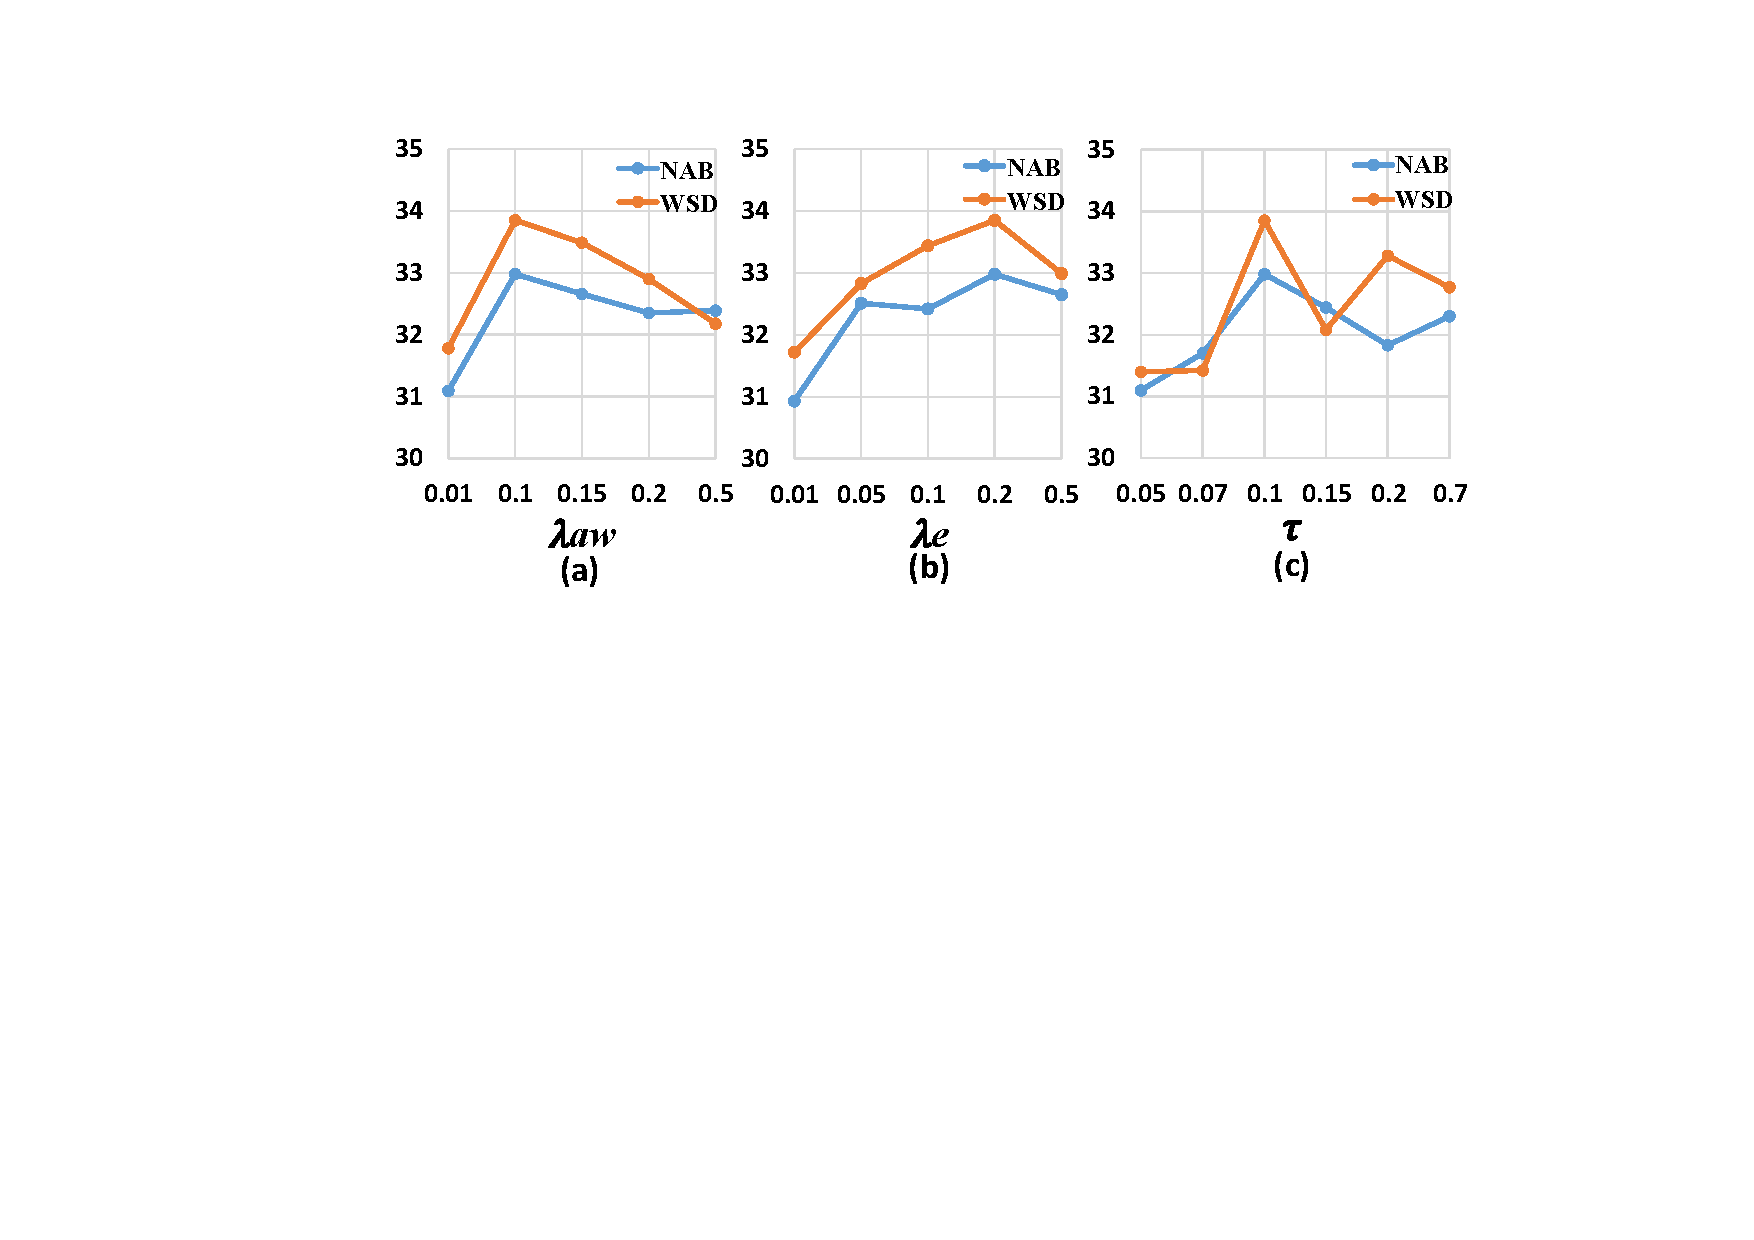
\includegraphics[width=1\linewidth]{IMG/img5.pdf}
    \caption{Hyperparameter analysis of $\lambda_{aw}, \lambda_{e}$, and $\tau$ in Terms of VUS-PR (\%)}
    \label{fig:img5}
\end{figure}
\begin{figure}[tb!]
    \centering
    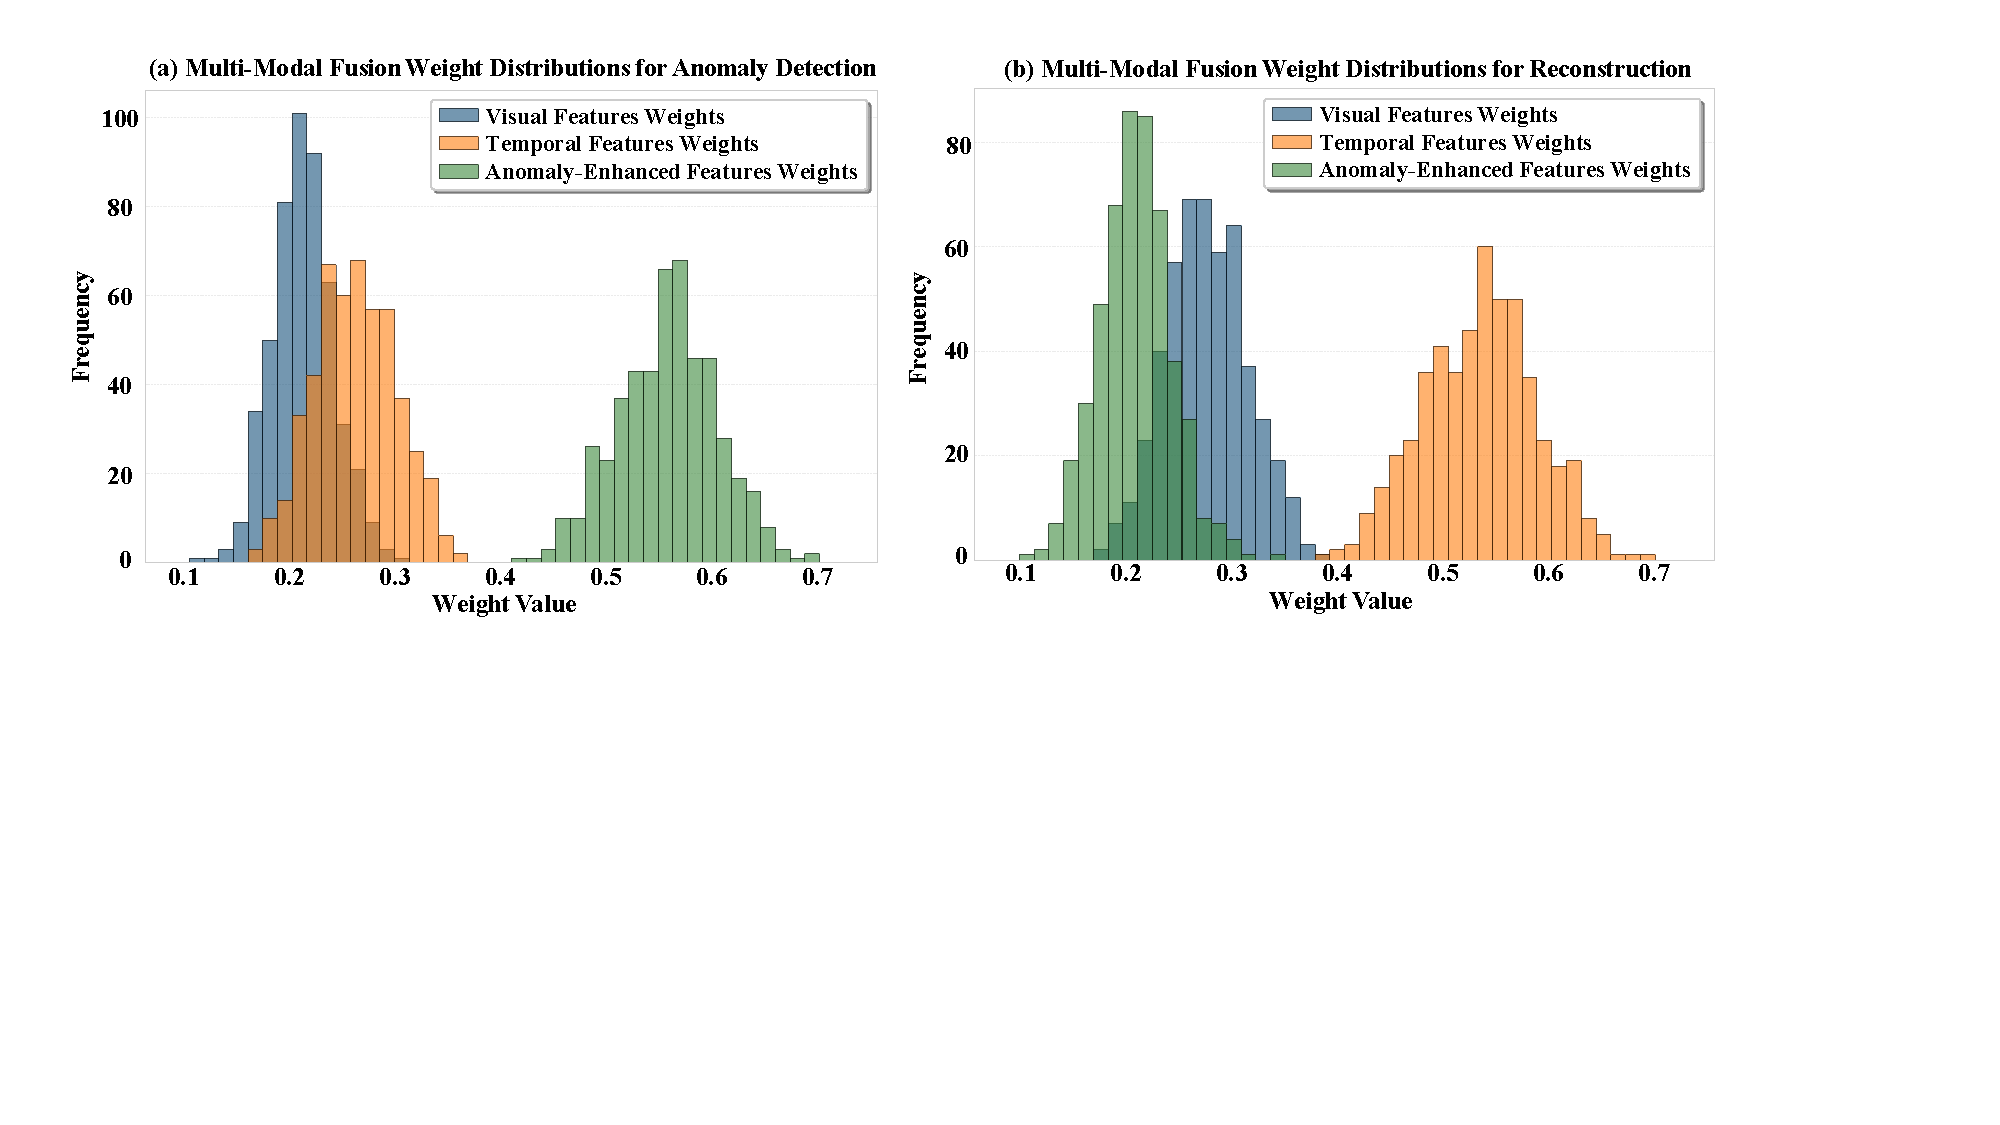
\includegraphics[width=1\linewidth]{IMG/img6.pdf}
    \caption{Visualization of fusion weights on the univariate datasets.}
    \label{fig:img6}
\end{figure}

\begin{figure*}[t!]
    \centering
    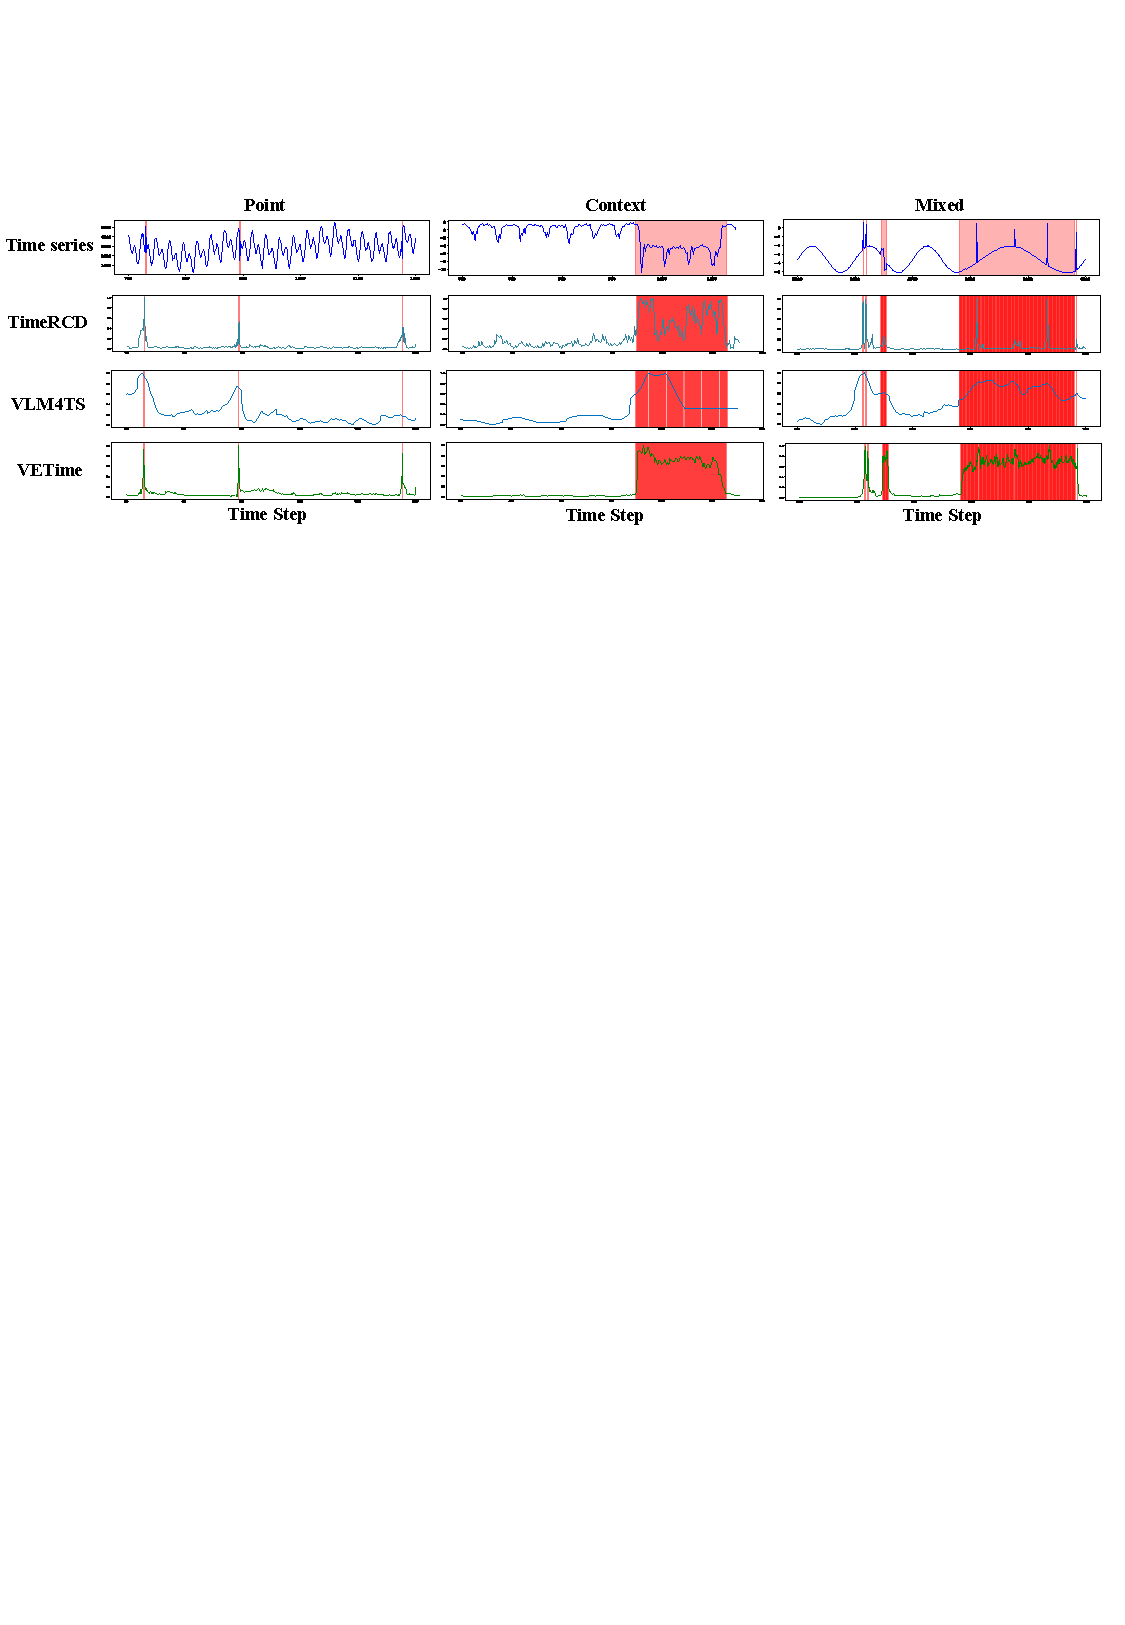
\includegraphics[width=0.9\linewidth]{IMG/img7.pdf}
     \caption{Qualitative comparison of anomaly detection results. The top row displays the original time series data as blue lines and highlights ground-truth anomalies using red shaded regions. The subsequent rows illustrate the anomaly scores generated by TimeRCD, VLM4TS, and VETime.}
    \label{fig:img7}
\vspace{-0.8em}
\end{figure*}

\vspace{-0.5em}
\section{Conclusion}
We propose VETime, which synergizes temporal sensitivity and global visual context. To bridge the gap between heterogeneous modalities, we introduce a Reversible Image Conversion method combined with Patch-Level Temporal Alignment. Furthermore, by leveraging Anomaly Window Contrastive Learning and Task-Adaptive Multi-Modal Fusion, the model addresses the limitations of unimodal approaches in capturing diverse anomaly patterns. Extensive experiments verify that VETime consistently outperforms state-of-the-art baselines in zero-shot scenarios. Future work will incorporate textual modalities to enhance interpretability, evolving the framework to detect anomalies and provide semantic explanations for their underlying causes.
% \paragraph{Limitation and Future Work.}

\nocite{langley00}

\bibliography{ref}
\bibliographystyle{icml2026}

%%%%%%%%%%%%%%%%%%%%%%%%%%%%%%%%%%%%%%%%%%%%%%%%%%%%%%%%%%%%%%%%%%%%%%%%%%%%%%%
%%%%%%%%%%%%%%%%%%%%%%%%%%%%%%%%%%%%%%%%%%%%%%%%%%%%%%%%%%%%%%%%%%%%%%%%%%%%%%%
% APPENDIX
%%%%%%%%%%%%%%%%%%%%%%%%%%%%%%%%%%%%%%%%%%%%%%%%%%%%%%%%%%%%%%%%%%%%%%%%%%%%%%%
%%%%%%%%%%%%%%%%%%%%%%%%%%%%%%%%%%%%%%%%%%%%%%%%%%%%%%%%%%%%%%%%%%%%%%%%%%%%%%%

\newpage
\appendix
\onecolumn

\section{Multivariate Model Adaptations}\label{appendix:Multivariate}
In the multivariate setting, we adapt the model as follows:

For multivariate time series input, we extend the aforementioned univariate \textbf{Reversible Image Conversion} to construct a unified three-channel heatmap representation. Specifically, each variable is first decomposed via Seasonal-Trend decomposition, and subsequently transformed through a variable-specific Gamma correction coefficient to apply differentiated non-linear mappings. This strategy enhances inter-variable discriminability in the visual domain by adapting to their distinct statistical distributions. The resulting individual heatmaps are then concatenated along the temporal dimension to form an integrated multivariate heatmap of size $ 1 \times (N_v L) \times 3 $ , where   $ N_v $  denotes the number of variables and $ L $ the temporal length per variable. Finally, this composite representation undergoes the same folding and scaling operations as described in the main text, yielding a consistent and unified visual input.

Regarding \textbf{Patch-Level Temporal Alignment}, the folding and scaling operations applied to the image features remain unchanged in the multivariate setting, the output is $\hat{F}_{V} \in \mathbb{R}^{N_{TS} \times N_v \times D_V}$. However, we inject an identical positional encoding vector $E_{POS}$ into the token sequence of each variable. Furthermore, we adapt the self-attention mechanism by leveraging the any-variate attention \cite{woo2024moirai}, which processes each variable’s temporal dynamics correction independently. Formally, the output are formulated as  $ F_{V} \in \mathbb{R}^{(N_{TS} N_v) \times D_{TS}} $. This design enables the model to separately reorganize the temporal order of features for each variable.

The \textbf{Anomaly Window Contrastive Learning} objective is applied independently to the feature sequence of each variable. Specifically, for every variable, we construct its own anomaly context window and perform positive/negative sample selection within its own temporal trajectory.

Finally, the \textbf{Task-Adaptive Multi-Modal Fusion} module remains unmodified in the multivariate setting, preserving its original architecture and functionality.

\section{Experimental Details}\label{appendix:B}
\subsection{Benchmark Datasets}\label{appendix:data_details}

Our evaluation uses a selection of datasets from one primary source, the TSB-AD benchmark by \cite{liu2024elephant}.

\begin{itemize}
    \item \textbf{Univariate Datasets}: We utilize a diverse collection of univariate datasets including IOPS, MGAB, NAB, NEK, Power, SED, TODS, UCR, and YAHOO.
    \item \textbf{Multivariate Datasets}: For multivariate anomaly detection, we use the SWaT, SMAP, SMD, MSL, and PSM datasets. These are sourced from industrial control systems and spacecraft telemetry, presenting complex, multi-dimensional dependencies.
\end{itemize}

The specific characteristics of these datasets, including their domain, number of time series (TS), average length, and anomaly ratio, are summarized in Table~\ref{tab:univariate_datasets} and Table~\ref{tab:multivariate_datasets}.

\begin{table}[h!]
\centering
\caption{Univariate Datasets}\label{tab:univariate_datasets}
\begin{tabular}{lllll}
\toprule
\textbf{Name} & \textbf{Domain} & \textbf{\#TS} & \textbf{Avg Length} & \textbf{AR (\%)} \\
\midrule
UCR & Misc. & 228 & 67818.7 & 0.6 \\
NAB & Web & 28 & 5099.7 & 10.6 \\
YAHOO & Web & 259 & 1560.2 & 0.6 \\
IOPS & Operations & 17 & 72792.3 & 1.3 \\
MGAB & Sensor & 9 & 97777.8 & 0.2 \\
SED & Energy & 3 & 23332.3 & 4.1 \\
TODS & Traffic & 15 & 5000.0 & 6.3 \\
NEK & Weather & 9 & 1073.0 & 8.0 \\
Power & Power Grid & 1 & 35040.0 & 8.5 \\
Stock&Stock&20&15000.0&9.4\\
WSD&Web&111&17444.5&0.6\\
\bottomrule
\end{tabular}
\end{table}

\begin{table}[h!]
\centering
\caption{Multivariate Datasets}\label{tab:multivariate_datasets}
\begin{tabular}{lllll}
\toprule
\textbf{Name} & \textbf{Domain} & \textbf{\#TS} & \textbf{Avg Length} & \textbf{AR (\%)} \\
\midrule
MSL & Space & 16 & 3119.4 & 5.1 \\
PSM & Sensor & 1 & 217624.0 & 11.2 \\
SMAP & Space & 27 & 7855.9 & 2.9 \\
SMD & Server & 22 & 25466.4 & 3.8 \\
SWaT & ICS & 2 & 207457.5 & 12.7 \\
\bottomrule
\end{tabular}
\end{table}

\subsection{Baselines}\label{appendix:baselines}

\textbf{Zero-Shot Models:} These models are pre-trained on large-scale datasets and can be applied directly to new time series without fine-tuning.

\begin{itemize}
    \item \textbf{Time-RCD}: This model, from the paper by \citep{lan2025foundationmodelszeroshottime}, is a pre-trained general anomaly detector. We set the window size to 5000 and patch size is 16.
    \item \textbf{DADA}: This model, from the paper by \citep{shentu2024towards}, is a pre-trained general anomaly detector. We set the window size to 100.
    \item \textbf{TS-Pulse}: An IBM foundation model that uses a TSMixer architecture \citep{ekambaram2025tspulse}. It is pre-trained on a massive corpus for multi-task applications, including anomaly detection. Following the suggestion from the paper, we set the window size with a length of 96.
    \item \textbf{MOMENT}: A foundation model that utilizes a patch-based pre-training strategy to learn rich representations from diverse time series data \citep{goswami2024moment}. We use a window size of 64.
    \item \textbf{TimesFM}: A decoder-only transformer model from Google trained on a large time series corpus using a patching strategy, enabling strong zero-shot generalization \citep{das2024decoder}. We set the window size to 96.
    \item \textbf{Chronos}: A generative model that frames time series analysis as a language modeling task, using a transformer-based architecture to learn and predict time series values \citep{ansari2024chronos}. Its window size is 100.
    \item \textbf{Time MOE}: A decoder-only transformer model with a sparse Mixture-of-Experts (MoE) architecture. It is pre-trained on a large time series corpus for forecasting and multi-task learning \citep{shi2024time}. We set the window size to 96.
\end{itemize}

\textbf{Full-Shot Models:} These models require training on the target dataset.

\begin{itemize}
    \item \textbf{TranAD}: A transformer-based model that uses a reconstructive approach to detect anomalies by comparing original and reconstructed time series \citep{tuli2022tranad}. It is configured with a window size of 10.
    \item \textbf{USAD}: An autoencoder-based model that employs an adversarial training mechanism to enhance its reconstruction capability and anomaly detection \citep{audibert2020usad}. We set the window size to 100.
    \item \textbf{OmniAnomaly}: A deep learning model that uses a Variational Autoencoder (VAE) with a Gated Recurrent Unit (GRU) to learn normal patterns and detect deviations \citep{su2019robust}. The model is configured with a window size of 100.
    \item \textbf{LOF}: A traditional statistical method that measures the local deviation of a data point from its neighbors, identifying anomalies with lower local density \citep{breunig2000lof}. For univariate datasets, we set n neighbors to 50, and for multivariate, we set n neighbors to 50 with metric as euclidean.
    \item \textbf{IForest}: An ensemble of Isolation Trees that isolates anomalies based on the number of random partitions required to separate them from the rest of the data \citep{liu2008isolation}. For univariate datasets, we set n estimators to 200, and for multivariate, we set n estimators to 25 and max features to 0.8.
\end{itemize}

\textbf{Vision-based Models} These models use powerful pre trained models for temporal anomaly detection without the need for additional training.

\begin{itemize}
    \item \textbf{VIT4TS}: A lightweight anomaly screening module that uses a pretrained Vision Transformer to encode time series rendered as line plots from overlapping sliding windows (window length 224, stride 56) and computes cross-window patch-level dissimilarity against a median normal reference to generate high-resolution anomaly heatmaps without fine-tuning\citep{he2025harnessing} .
    \item \textbf{VLM4TS}: A zero-shot time series anomaly detection framework that combines a pretrained vision-language model (GPT-4o) with a two-stage pipeline. It first using ViT4TS for candidate localization and then prompting the full VLM with a global line plot and textual candidate list to perform semantic validation and refinement of anomalies under a unified multimodal reasoning process\citep{he2025harnessing}.
    \item \textbf{VisualTimeAnomaly}: It converts univariate and multivariate time series into line-plot images (TSIs) and uses off-the-shelf multimodal large language models (GPT-4o) on point-wise, range-wise, and variate-wise anomaly detection tasks. \citep{xu2025can}.
    \item \textbf{AnomLLM}: It involves plotting time series data as line charts and leverages GPT-4o-mini's visual multimodal capabilities to detect anomaly patterns by directly "viewing" the plot, rather than analyzing numerical text.\cite{zhou2024llmsunderstandtimeseries}.
\end{itemize}

\subsection{Evaluation Metric Calculations}\label{appendix:metric}

Our performance evaluation is conducted using four metrics: Affiliation-F1, Temporal-F1 ($F1_T$), Standard-F1 ($F1$), and Volume Under Surface - Precision/Recall(VUS-PR). 

\begin{itemize}

\item \textbf{Standard-F1} is a widely used metric that provides a harmonic mean of precision and recall. It is calculated using point-wise True Positives (TP), False Positives (FP), and False Negatives (FN).
\item \textbf{F1-T} as described by \cite{sarfraz2024position}, is a range-based metric that evaluates anomaly detection performance by considering the temporal context of anomalies. It is a variant of the F1-score that addresses common issues in time series evaluation, such as overlapping predictions and temporal proximity.
\item \textbf{Affiliation-F1} is a distance-based metric that measures the "affiliation" or proximity between the ground truth and predicted anomaly points. It is designed to be less sensitive to minor temporal shifts in the predicted anomalies. The score is calculated by finding the optimal one-to-one mapping between the ground truth and detected anomalies and then computing the F1-score based on these affiliations \citep{huet2022local}.
\item \textbf{VUS-PR} is a threshold-independent, parameter-free metric for time series anomaly detection. Unlike point-wise metrics, VUS-PR is robust to time lags and measures the area under a 3D surface plot of precision, recall, and a buffer parameter \citep{paparrizos2022volume}. It addresses the limitations of standard F1 scores by creating a continuous buffer region around each anomaly, thus providing a more reliable and nuanced evaluation of model performance.
\end{itemize}

\subsection{Implementation Details} \label{AppendixC4}

\paragraph{Implementation:}
The input time series is divided into patches of size 16. The visual and temporal backbone employ the encoder of the frozen MAE\cite{chen2024visionts} and pre-trained  transformer architecture\cite{lan2025foundationmodelszeroshottime}, respectively, with feature dimensions of 768 and 512. These are projected to a shared dimension of 512 during fusion. Hyper-parameters $\lambda_{aw}, \lambda_{e}$, and $\tau$ are fixed at $0.1$, $0.2$, and $0.1$. The model is trained on synthetic data \cite{lan2025foundationmodelszeroshottime} with a batch size of 32, using AdamW optimizer with a learning rate of 5e-4 and a weight decay of 1e-5, for up to 25 epochs, with early stopping if no improvement is observed for 4 consecutive epochs. 

\paragraph{Encoders:} Our framework leverages a dual-encoder architecture to process heterogeneous modalities.
\begin{itemize}
\item \textbf{Vision Encoder:} We adopt the encoder from a pre-trained Masked Autoencoder (MAE) as our visual backbone. Specifically, we utilize the lightweight ViT-Base architecture to extract robust semantic representations from the converted time-series images.
\item \textbf{Time-Series Encoder:} We employ a classical Transformer architecture consisting of learnable positional encodings, a stack of Encoder layers with Multi-Head Self-Attention (MHSA), and Feed-Forward Networks (FFN), followed by Layer Normalization. This encoder features 8 transformer layers, each with 8 attention heads. We initialize our encoder using the pre-trained weights from Time-RCD \cite{lan2025foundationmodelszeroshottime}.
To achieve parameter-efficient adaptation, we apply Low-Rank Adaptation (LoRA) to fine-tune the linear projection matrices within both the Attention mechanism and the FFN modules. Specifically, we set the LoRA rank r = 8 and the scaling hyperparameter $\alpha = 16$, resulting in a scaling factor of $\alpha/r = 2$. LoRA adapters are inserted into all trainable linear layers of the encoder, while the original pre-trained weights remain frozen during fine-tuning.
\end{itemize}


\paragraph{Loss:} \label{appx.loss}
The task-specific features $F_{AD}$ and $F_{Rec}$, derived from the fusion module, are passed through dedicated prediction heads to generate the final anomaly probabilities and reconstructed sequence:
\begin{equation}
\hat{y}_t = Softmax(\text{MLP}_{AD}(F_{AD})), \quad \hat{x}_t = \text{MLP}_{Rec}(F_{Rec})
\end{equation}
where $\hat{Y} \in \mathbb{R}^{L}$ denotes the sequence of anomaly probabilities $\{\hat{y}_t\}_{t=1}^{L}$, and $\hat{X} \in \mathbb{R}^{L}$ represents the reconstructed time series $\{\hat{x}_t\}_{t=1}^{L}$. $\text{MLP}_{AD}$ and $\text{MLP}_{Rec}$ act as the anomaly classifier and reconstruction projector, respectively. $Softmax(\cdot)$ is the Softmax function used to map the logits to the range $[0,1]$ for probability estimation.

The model is trained end-to-end using a composite loss function that balances classification accuracy, reconstruction quality, and feature alignment:
\begin{equation}
\mathcal{L}_{total} = \mathcal{L}_{BCE} + \mathcal{L}_{MSE} + \lambda_{aw} \mathcal{L}_{aw} + \lambda_{e} \mathcal{L}_{e}
\end{equation}
where $\mathcal{L}_{BCE}$ denotes the Binary Cross-Entropy loss for anomaly classification:
\begin{equation}
\mathcal{L}_{BCE} = - \frac{1}{L} \sum_{t=1}^{L} \left[ y_t \log(\hat{y}_t) + (1 - y_t) \log(1 - \hat{y}_t) \right]
\end{equation}
where $L$ is the sequence length, $y_t \in \{0,1\}$ is the ground truth anomaly label at time step $t$, and $\hat{y}_t$ is the predicted anomaly probability. $\mathcal{L}_{MSE}$ represents the Mean Squared Error loss supervising sequence reconstruction:
\begin{equation}
\mathcal{L}_{MSE} = \frac{1}{L} \sum_{t=1}^{L} \| x_t - \hat{x}_t \|_2^2
\end{equation}
where $x_t$ and $\hat{x}_t$ represent the original and reconstructed input values at time step $t$, respectively.

\paragraph{Training Data:} To ensure robust zero-shot generalization, we constructed a large-scale synthetic dataset comprising a total of 0.5 billion data points refer to \cite{lan2025foundationmodelszeroshottime}. The dataset features sequences with variable lengths ranging from 500 to 10,000 time steps. It is designed to cover a diverse spectrum of anomaly patterns, encompassing both long-term context deviations (e.g., trend shifts) and fine-grained local anomalies (e.g., point outliers).



\begin{table*}[t!]
\centering
\caption{Performance of VETime against zero-shot and full-shot baselines. VETime operates in a strictly zero-shot capacity in all comparisons. Best result is in \textcolor{red}{red}, second-best is in \textcolor{blue}{blue}. Asterisked (*) results are excluded from ranking due to data leaking.}
\label{tab:mainm}
\small
\begin{tabular}{l|l|ccccc|c|c}
    \hline
    \multirow{2}{*}{\textbf{Metric}} & \multirow{2}{*}{\textbf{Model}} & \multicolumn{5}{c|}{\textbf{Multivariate Datasets}} & \textbf{Total} & \textbf{Total} \\
    \cline{3-7}
    & & \textbf{MSL} & \textbf{PSM} & \textbf{SMAP} & \textbf{SMD} & \textbf{SWaT} & \textbf{1st} & \textbf{2nd} \\
    \hline
    \multicolumn{8}{c}{\textbf{Zero-Shot Models}} \\
    \hline
    \multirow{6}{*}{Affiliation-F1} 
    & VETime & \textcolor{red}{\textbf{87.02}} & 77.27 & \textcolor{blue}{\textbf{87.06}} & \textcolor{blue}{\textbf{88.94}} & \textcolor{blue}{\textbf{75.45}} & 01 & 03 \\
    & TimeRCD &  \textcolor{blue}{\textbf{81.16}} & \textcolor{red}{\textbf{81.61}} & \textcolor{red}{\textbf{87.73}} & \textcolor{red}{\textbf{92.58}} & 71.55 & 03 & 01 \\
    & DADA† & 76.57 & \textcolor{blue}{\textbf{81.27}} & 76.92 & 83.74 & \textcolor{red}{\textbf{76.18}} & 01 & 01 \\
    & TS-Pulse & 70.14 & 70.28 & 69.21 & 68.21 & 71.18 & 00 & 00 \\
    & MOMENT† & 74.55\rlap{*} & 65.79 & 77.42 \rlap{*}  & 74.00 \rlap{*}  & 70.17 & 00 & 00 \\
    & Time MOE & 69.85 & 54.74 & 74.38 & 69.97 & 64.37 & 00 & 00 \\
    \hline
    \multirow{6}{*}{F1\_T} 
    & VETime & \textcolor{red}{\textbf{43.52}} & \textcolor{red}{\textbf{39.06}} & \textcolor{red}{\textbf{45.52}} & \textcolor{blue}{\textbf{53.36}} & \textcolor{red}{\textbf{39.94}} & 04 & 01 \\
    & TimeRCD & \textcolor{blue}{\textbf{42.47}} & \textcolor{blue}{\textbf{37.98}} & \textcolor{blue}{\textbf{33.74}} & \textcolor{red}{\textbf{53.91}} & 30.28 & 01 & 03 \\
    & DADA† & 34.58 & 31.84& 30.42 & 40.80 & \textcolor{blue}{\textbf{35.13}} & 00 & 01 \\
    & TS-Pulse & 23.57 & 25.39 & 12.34 & 09.15 & 28.58 & 00 & 00 \\
    & MOMENT† & 25.97 \rlap{*}  & 27.77 & 17.93 \rlap{*}  & 28.68 \rlap{*}  & 28.76 & 00 & 00 \\
    & Time MOE & 23.92 & 26.82 & 14.22 & 19.90 & 30.11 & 00 & 00 \\
    \hline
    \multirow{6}{*}{Standard-F1} 
    & VETime & \textcolor{red}{\textbf{35.24}} & \textcolor{red}{\textbf{27.05}} & \textcolor{red}{\textbf{32.16}} & \textcolor{red}{\textbf{51.41}} & \textcolor{red}{\textbf{55.87}} & 05 & 00 \\
    & TimeRCD & \textcolor{blue}{\textbf{30.66}} & \textcolor{blue}{\textbf{26}} & \textcolor{blue}{\textbf{30.48}} & \textcolor{blue}{\textbf{44.89}} & 28.73 & 00 & 04 \\ 
    & DADA† & 22.13 & 24.07 & 26.75& 34.94 & \textcolor{blue}{\textbf{34.78}} & 00 & 01 \\
    & TS-Pulse & 12.56 & 22.31 & 07.44 & 08.00 & 23.84 & 00 & 00 \\
    & MOMENT† & 14.43 \rlap{*}  & 23.83 & 12.92 \rlap{*}  & 29.78 \rlap{*}  & 21.30 & 00 & 00 \\
    & Time MOE & 12.85 & \textcolor{blue}{\textbf{24.80}} & 09.01 & 21.62 & 23.58 & 00 & 00 \\
    \hline
    \multirow{6}{*}{VUS-PR} 
    & VETime & \textcolor{red}{\textbf{30.51}} & \textcolor{red}{\textbf{23.86}} & \textcolor{red}{\textbf{23.70}} & \textcolor{red}{\textbf{48.21}} & \textcolor{red}{\textbf{42.93}} & 05 & 00 \\
    & TimeRCD & \textcolor{blue}{\textbf{20.45}} & \textcolor{blue}{\textbf{18.69}} & \textcolor{blue}{\textbf{22.68}} & \textcolor{blue}{\textbf{37.03}} & 17.58 & 00 & 04 \\ 
    & DADA† & 12.74 & 17.17 & 20.02 & 25.98 & \textcolor{blue}{\textbf{21.13}} & 00& 01 \\
    & TS-Pulse & 07.41 & 14.48 & 03.99 & 04.56 & 15.67 & 00 & 00 \\
    & MOMENT† & 09.32 \rlap{*}  & 16.48 & 08.97 \rlap{*}  & 15.96 \rlap{*}  & 14.90 & 00 & 00 \\
    & Time MOE & 07.82 & 15.68 & 04.98 & 11.12 & 16.20 & 00 & 00 \\
    \hline
    \multicolumn{7}{l}{\textbf{VETime Grand Total (Zero-Shot)}} & \textbf{15} & \textbf{4} \\
    \hline
    \multicolumn{8}{c}{\textbf{Full-Shot Models}} \\
    \hline
    \multirow{5}{*}{Affiliation-F1} 
    & VETime & \textcolor{red}{\textbf{87.02}} & \textcolor{red}{\textbf{77.27}} & \textcolor{blue}{\textbf{87.06}} & \textcolor{blue}{\textbf{88.94}} & \textcolor{red}{\textbf{75.45}} & 03 & 02 \\
    & TranAD & 79.91 & \textcolor{blue}{\textbf{73.83}} & 87.39 & \textcolor{red}{\textbf{92.20}} & \textcolor{blue}{\textbf{75.37}} & 01 & 01 \\
    & USAD & 81.86 & 57.86 & 87.25 & 85.09 & 75.06 & 01 & 00 \\
    & OmniAnomaly & 83.15 & 58.17 & \textcolor{red}{\textbf{91.38}} & 85.82 & 73.39 & 03 & 02 \\
    & LOF & \textcolor{blue}{\textbf{84.35}} & 61.98 & 63.32 & 64.13 & 56.34 & 00 & 01 \\
    \hline
    \multirow{5}{*}{F1\_T} 
    & VETime & 43.52& \textcolor{red}{\textbf{39.06}} & \textcolor{blue}{\textbf{45.52}} & \textcolor{red}{\textbf{53.36}} & 39.94 & 02 & 01 \\
    & TranAD & 39.42 & 25.49 & 29.12 & 37.98 & \textcolor{blue}{\textbf{49.58}} & 00 & 01 \\
    & USAD & \textcolor{blue}{\textbf{48.71}} & 28.96 & 43.94 & 50.41 & \textcolor{red}{\textbf{50.41}} & 01 & 01 \\
    & OmniAnomaly & \textcolor{red}{\textbf{49.36}} & \textcolor{blue}{\textbf{30.42}} & \textcolor{red}{\textbf{46.63}} & \textcolor{blue}{\textbf{51.84}} & 46.64 & 02 & 02 \\
    & LOF & 38.97 & 25.58 & 21.81 & 10.13 & 30.62 & 00 & 00 \\
    \hline
    \multirow{5}{*}{Standard-F1} 
     & VETime & 35.24 & 27.05 & 32.16 & 51.41 & 55.87 & 00 & 00 \\
    & TranAD & 29.60 & 25.63 & 25.11 & 43.99 & \textcolor{blue}{\textbf{61.86}} & 00 & 01 \\
    & USAD & \textcolor{blue}{\textbf{38.71}} & \textcolor{blue}{\textbf{28.41}} & \textcolor{blue}{\textbf{38.66}} & \textcolor{blue}{\textbf{53.06}} & \textcolor{red}{\textbf{62.82}} & 01 & 04 \\
    & OmniAnomaly & \textcolor{red}{\textbf{39.10}} & \textcolor{red}{\textbf{30.43}} & \textcolor{red}{\textbf{40.50}} & \textcolor{red}{\textbf{57.06}} & 55.93 & 04 & 00 \\
    & LOF & 30.65 & 18.80 & 18.70 & 08.41 & 29.08 & 00 & 00 \\
    \hline
    \multirow{5}{*}{VUS-PR} 
    & VETime & \textcolor{blue}{\textbf{30.51}} & \textcolor{red}{\textbf{23.86}} & 23.70 & \textcolor{red}{\textbf{48.21}} & 42.93 & 02 & 01 \\
    & TranAD & 14.78 & 16.49 & 13.37 & 28.34 & \textcolor{red}{\textbf{47.37}} & 01 & 00 \\
    & USAD & 29.95 & 17.59 & \textcolor{blue}{\textbf{26.37}} & 34.53 & \textcolor{blue}{\textbf{44.73}} & 00 & 02 \\
    & OmniAnomaly & \textcolor{red}{\textbf{31.57}} & \textcolor{blue}{\textbf{18.58}} & \textcolor{red}{\textbf{28.07}} & \textcolor{blue}{\textbf{37.44}} & 42.97 & 02 & 02 \\
    & LOF & 24.67 & 13.58 & 10.59 & 04.40 & 14.50 & 00 & 00 \\
    \hline
    \multicolumn{7}{l}{\textbf{VETime Grand Total (Full-Shot)}} & \textbf{7} & \textbf{4} \\
    \hline
\end{tabular}
\end{table*}

\section{Additional Experimental Results}\label{appendix:C}

\subsection{Multivariate Experiments}\label{appendix:C1}
As shown in Table \ref{tab:mainm}, VETime establishes a new state-of-the-art in zero-shot anomaly detection, demonstrating overwhelming superiority over existing baselines (e.g., TimeRCD, DADA) by securing the top rank in 15 comparison instances. It consistently achieves the highest performance in critical metrics, particularly VUS-PR, across all datasets, which highlights its stability and precision independent of threshold selection. Remarkably, despite operating strictly in a zero-shot capacity, VETime exhibits exceptional generalization, frequently matching or even surpassing fully supervised full-shot models like TranAD and USAD (e.g., on MSL and SMAP). This cross-paradigm success validates the effectiveness of our proposed multi-modal alignment and fusion mechanism, proving its ability to capture universal discriminative anomaly patterns without the need for domain-specific training.

\begin{table}[t!]
\centering
\small
\caption{Ablation study grouped by different vision encoder. Metrics: Affiliation-F1 (\%) and VUS-PR (\%).}
\label{tab:ablation_vision}
\begin{tabular}{
    >{\centering\arraybackslash}m{0.7cm}   % Model (col1)
    >{\centering\arraybackslash}m{3.3cm}   % Component (col2)
    *{6}{>{\centering\arraybackslash}m{1.4cm}}  % 6 metric columns
}
\toprule
\multirow{3}{*}{\textbf{Model}} & \multirow{3}{*}{\textbf{Size}} & \multicolumn{2}{c}{\textbf{NAB}} & \multicolumn{2}{c}{\textbf{WSD}} & \multicolumn{2}{c}{\textbf{YAHOO}} \\
\cmidrule(lr){3-4} \cmidrule(lr){5-6} \cmidrule(lr){7-8}
 &  & \makecell{Affiliation\\-F1} & \makecell{VUS\\-PR} & \makecell{Affiliation\\-F1} & \makecell{VUS\\-PR} & \makecell{Affiliation\\-F1} & \makecell{VUS\\-PR} \\
\midrule
Vit (Base) & 85.64M  & 88.42 & \textcolor{blue}{\textbf{32.72}} & 93.01 & 30.90 & 95.87 & 86.12 \\
MAE (Base) & 85.64M & \textcolor{blue}{\textbf{88.57}} & \textcolor{red}{\textbf{32.98}} & \textcolor{red}{\textbf{94.31}} & \textcolor{blue}{\textbf{33.85}} & \textcolor{red}{\textbf{97.15}} & \textcolor{red}{\textbf{88.61}} \\
MAE (Large) &  303.10M  & \textcolor{red}{\textbf{88.67}} & 31.54 & \textcolor{blue}{\textbf{93.94}} & \textcolor{red}{\textbf{34.10}} & \textcolor{blue}{\textbf{97.03}} & \textcolor{blue}{\textbf{87.20}} \\
\bottomrule
\end{tabular}
\end{table}

\subsection{Ablation Study on Vision Encoder}\label{appendix:C2}

\paragraph{Impact of vision backbones.}
To investigate the influence of the vision backbone on detection performance, we evaluate VETime with three vision encoders with different initialized pre-trained weights: ViT (Base) \cite{dosovitskiy2020image}, MAE (Base), and MAE (Large) \citep{he2022masked}. As shown in Table~\ref{tab:ablation_vision}, MAE-based encoders consistently outperform the standard ViT (Base), demonstrating the benefit of masked autoencoding pre-training for time-series anomaly detection—a task that inherently involves reconstructing and reasoning about corrupted or anomalous segments.
However, scaling up to MAE (Large) yields only marginal gains despite a 3.5× increase in parameters, and even degrades performance on YAHOO. In contrast, MAE (Base) delivers the best balance between performance, efficiency, and robustness across all three datasets. Therefore, we adopt MAE (Base) as the default vision encoder in our final VETime architecture.


\paragraph{Impact of the different imaging strategies.}
The ablation study in Table \ref{tab:ablation_vision2} systematically evaluates the contribution of each component in our reversible image conversion pipeline. Strategy A, which uses a simple line plot without any advanced encoding, achieves relatively low VUS-PR scores, indicating limited capacity to capture subtle anomaly patterns. Strategy B introduces multi-channel intensity mapping, significantly improving both Affiliation-F1 and VUS-PR across all datasets by leveraging RGB channels to encode trend and residual components jointly. This demonstrates that richer visual representations enhance anomaly detection sensitivity. Strategy C adds adaptive folding, further boosting performance on WSD (Affiliation-F1: 90.55\% → 92.30\%), suggesting that spatial reorganization via periodic folding helps preserve long-term temporal dependencies. However, its impact is less pronounced on shorter sequences like Yahoo. Strategy D incorporates dimension-aware scaling, which improves generalization by aligning input resolution to standard vision models while preserving waveform fidelity. Notably, the full model (Strategy E) achieves the highest scores across all metrics and datasets, confirming the synergistic effect of combining multi-channel encoding, adaptive folding, and dimension-aware scaling.
\begin{figure}
    \centering
    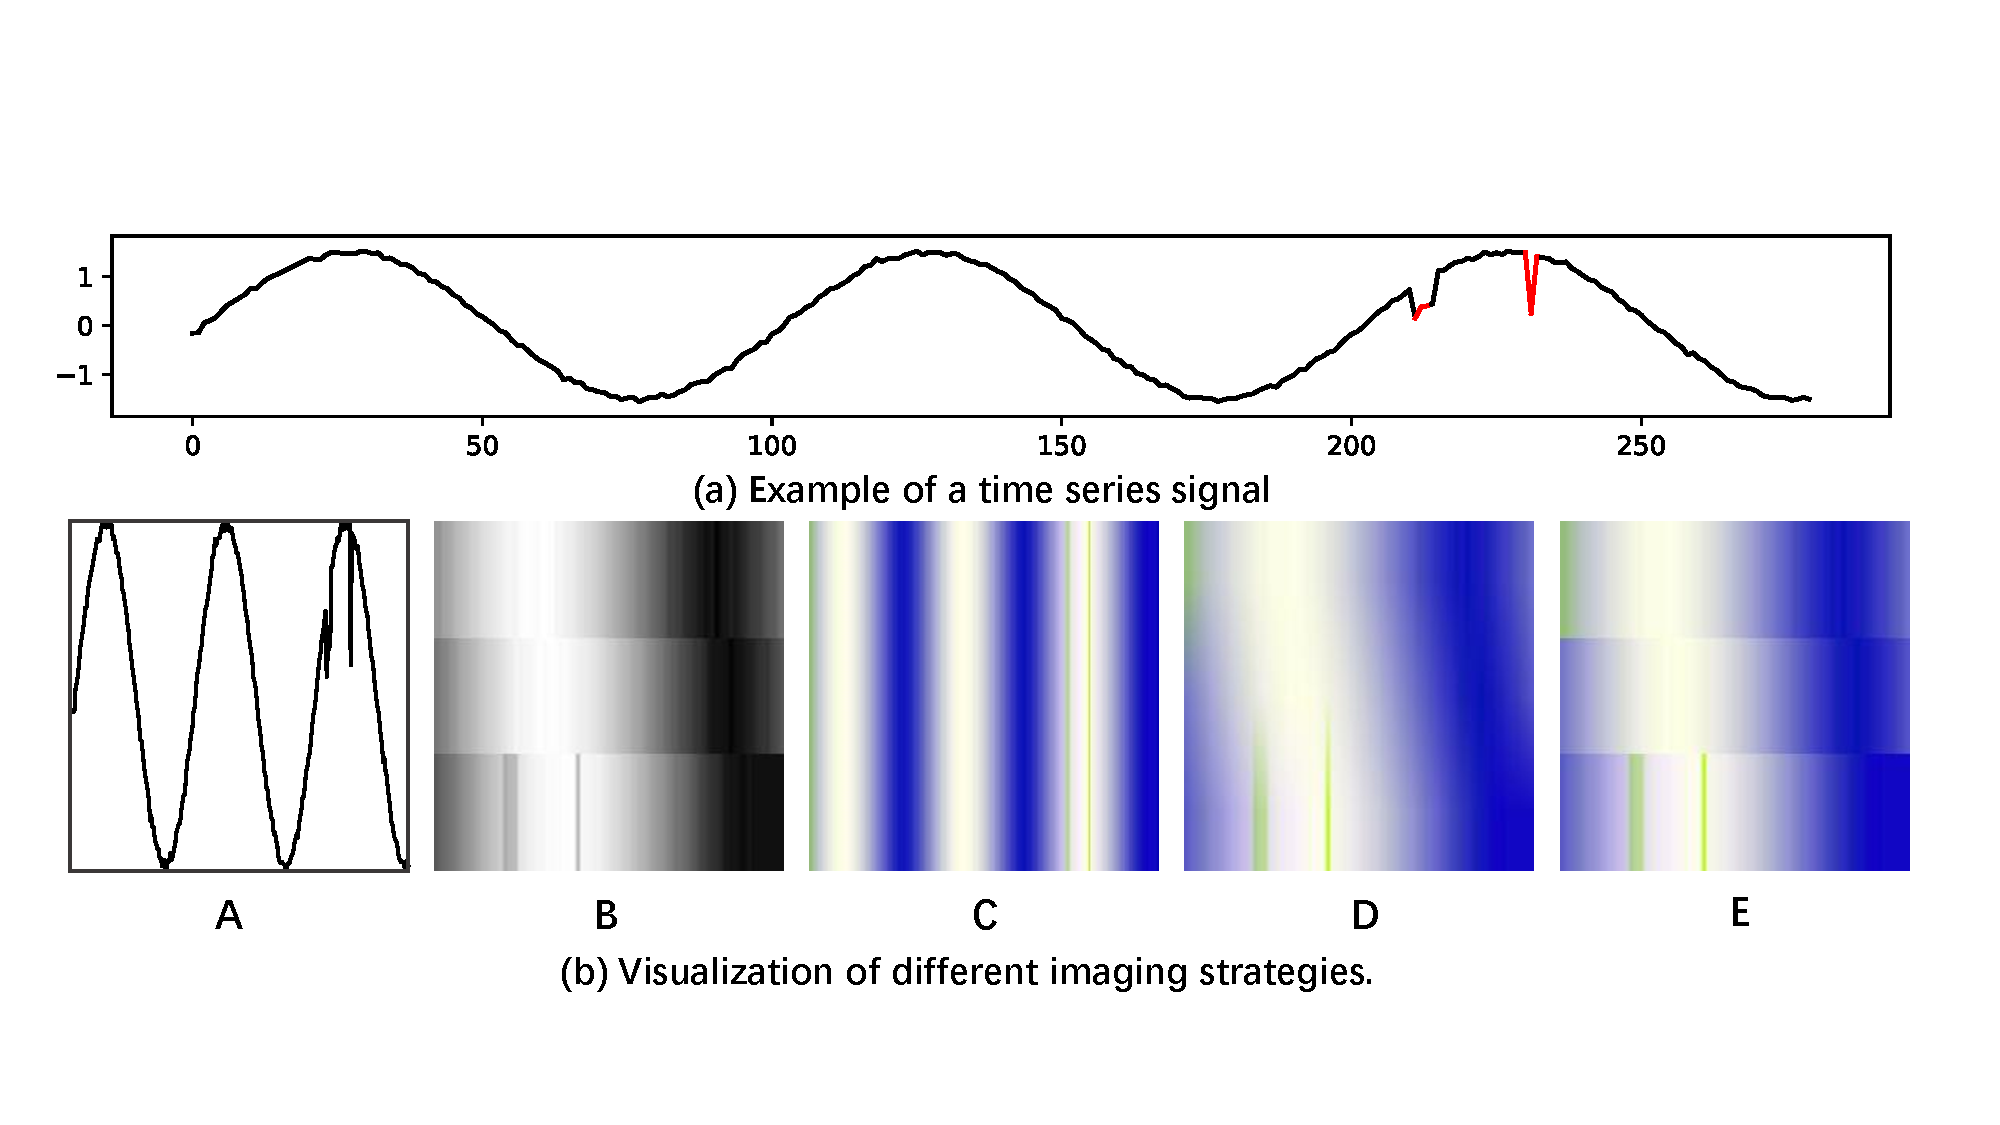
\includegraphics[width=1\linewidth]{IMG/img8.pdf}
    \caption{Visualization of different imaging strategies.}
    \label{fig:img8}
\end{figure}

\begin{table}[t!]
\centering
\small
\caption{Ablation study grouped by different imaging strategies in Figure \ref{fig:img8}. Metrics: Affiliation-F1 (\%) and VUS-PR (\%).}
\label{tab:ablation_vision2}
\begin{tabular}{
    >{\centering\arraybackslash}m{0.7cm}   % Model (col1)
    >{\centering\arraybackslash}m{3.3cm}   % Component (col2)
    *{6}{>{\centering\arraybackslash}m{1.4cm}}  % 6 metric columns
}
\toprule
\multirow{3}{*}{\textbf{Strategies}} & \multirow{3}{*}{\textbf{Description}} & \multicolumn{2}{c}{\textbf{NAB}} & \multicolumn{2}{c}{\textbf{WSD}} & \multicolumn{2}{c}{\textbf{YAHOO}} \\
\cmidrule(lr){3-4} \cmidrule(lr){5-6} \cmidrule(lr){7-8}
 &  & \makecell{Affiliation\\-F1} & \makecell{VUS\\-PR} & \makecell{Affiliation\\-F1} & \makecell{VUS\\-PR} & \makecell{Affiliation\\-F1} & \makecell{VUS\\-PR} \\
\midrule
A & Line plot (w/o Reversible Image Conversion)    & 83.85 & 24.05 & 88.01 & 18.71 & 94.81 & 82.53 \\
B & w/o Multi-Channel Intensity Mapping   & \textcolor{blue}{\textbf{86.47}} & 28.81 & 91.25 & \textcolor{blue}{\textbf{33.61}} & \textcolor{blue}{\textbf{96.53}} & \textcolor{blue}{\textbf{87.30}} \\
C & w/o Adaptive Folding    & 85.07 & 25.03 & 90.55 & 25.03 & 94.71 & 84.11 \\
D & w/o Dimension-Aware Scaling & 86.11 & \textcolor{blue}{\textbf{30.33}} & \textcolor{blue}{\textbf{92.30}} & 30.79 & 95.57 & 86.45 \\
E (Ours) & - & \textcolor{red}{\textbf{88.57}} & \textcolor{red}{\textbf{32.98}} & \textcolor{red}{\textbf{94.31}} & \textcolor{red}{\textbf{33.85}} & \textcolor{red}{\textbf{97.15}} & \textcolor{red}{\textbf{88.61}} \\
\bottomrule
\end{tabular}
\end{table}


\subsection{Full Ablation Study on each component}\label{appendix:C2}
To verify the effectiveness of each component in our proposed framework, we conducted a comprehensive ablation study on the NAB, WSD, and YAHOO datasets. Table \ref{tab:ablation_all} summarizes the results grouped by the three key modules: Patch-Level Temporal Alignment (PTA), Anomaly Window Contrastive Learning (AWCL), and Task-Adaptive Multi-Modal Fusion (TMF).


\begin{table}[t!]
\centering
\small
\caption{Ablation study grouped by model components: PTA (Patch-Level Temporal Alignment), AWCL (Anomaly Window Contrastive Learning), and TMF (Task-Adaptive Multi-Modal Fusion). Metrics: Affiliation-F1 (\%) and VUS-PR (\%).}
\label{tab:ablation_all}
\begin{tabular}{
    >{\centering\arraybackslash}m{0.7cm}   % Model (col1)
    >{\centering\arraybackslash}m{3.3cm}   % Component (col2)
    *{6}{>{\centering\arraybackslash}m{1.5cm}}  % 6 metric columns
}
\toprule
\multirow{3}{*}{\textbf{Model}} & \multirow{3}{*}{\textbf{Component}} & \multicolumn{2}{c}{\textbf{NAB}} & \multicolumn{2}{c}{\textbf{WSD}} & \multicolumn{2}{c}{\textbf{YAHOO}} \\
\cmidrule(lr){3-4} \cmidrule(lr){5-6} \cmidrule(lr){7-8}
 &  & \makecell{Affiliation\\-F1} & \makecell{VUS\\-PR} & \makecell{Affiliation\\-F1} & \makecell{VUS\\-PR} & \makecell{Affiliation\\-F1} & \makecell{VUS\\-PR} \\
\midrule
\multirow{3}{=}{PTA} 
& w/o adaptive folding       & 87.81 & 29.99 & 91.49 & 30.41 & 97.10 & 86.70 \\
& w/o positional encoding    & 88.16 & 30.27 & 92.29 & 31.18 & 97.25 & 86.81 \\
& w/o attention              & 85.69 & 29.88 & 91.57 & 29.46 & 96.92 & 85.53 \\
\midrule
\multirow{2}{=}{AWCL} 
& w/o inter-window contrast  & 86.69 & 31.17 & 92.85 & 30.54 & 97.15 & 87.29 \\
& w/o intra-window contrast  & 86.15 & 30.86 & 92.93 & 30.57 & 97.77 & 88.29 \\
\midrule
\multirow{3}{=}{TMF} 
& Concatenation             & 83.99 & 28.54 & 89.80 & 26.30 & 95.69 & 85.31 \\
& Addition                  & 85.07 & 29.52 & 90.11 & 26.39 & 96.86 & 85.72 \\
& w/o reconstruction head    & 86.96 & 28.44 & 90.87 & 28.63 & 96.88 & 86.58 \\
\bottomrule
\end{tabular}
\end{table}

\paragraph{Effect of Patch-Level Temporal Alignment (PTA).}
We investigated the contributions of adaptive folding, positional encoding, and the attention mechanism within the PTA module. As observed, removing the \textbf{attention mechanism} resulted in the most significant performance degradation across all datasets (e.g., Affiliation-F1 dropped to 85.69\% on NAB). This indicates that the attention mechanism is pivotal for capturing long-range dependencies and accurately aligning visual patches with temporal contexts. Furthermore, the exclusion of \textbf{adaptive folding} also led to a notable decline, validating its role in preserving intrinsic temporal structures during feature transformation. These results confirm that the complete PTA design is essential for ensuring fine-grained semantic correspondence.


\begin{table}[b!]
\centering
\small
\caption{Performance comparison under different types of anomalies.}
\label{tab:tab10}
\begin{tabular}{llccc}
\toprule
\textbf{Metric} & \textbf{Model} & \textbf{Local} & \textbf{Global} & \textbf{Mixed} \\
\midrule
\multirow{3}{*}{Affiliation-F1} 
& VETime    & \textcolor{red}{\textbf{93.20}} & \textcolor{red}{\textbf{91.79}} & \textcolor{red}{\textbf{87.78}} \\
& TimeRCD    & \textcolor{blue}{\textbf{74.84}}&\textcolor{blue}{\textbf{73.84}}&\textcolor{blue}{\textbf{73.03}}\\
& VLM4TS & 67.11&61.94&60.79
 \\

\midrule
\multirow{3}{*}{F1\_T} 
& VETime    & \textcolor{red}{\textbf{66.17}} & \textcolor{red}{\textbf{63.32}} & \textcolor{red}{\textbf{52.61}} \\
& TimeRCD    & \textcolor{blue}{\textbf{31.51}}&\textcolor{blue}{\textbf{54.06}}&	\textcolor{blue}{\textbf{42.12}} \\
& VLM4TS & 21.60&35.90&29.63 \\

\midrule
\multirow{3}{*}{Standard-F1} 
& VETime    & \textcolor{red}{\textbf{62.33}} & \textcolor{red}{\textbf{59.74}} & \textcolor{red}{\textbf{44.28}} \\
& TimeRCD    & \textcolor{blue}{\textbf{28.34}}&32.18&26.20\\
& VLM4TS & 23.15&\textcolor{blue}{\textbf{35.90}}&\textcolor{blue}{\textbf{34.52}} \\
\midrule
\multirow{3}{*}{VUS-PR} 
& VETime    & \textcolor{blue}{\textbf{59.33}} & \textcolor{red}{\textbf{57.59}} & \textcolor{red}{\textbf{44.61}} \\
& TimeRCD    & \textcolor{red}{\textbf{61.85}} & \textcolor{blue}{\textbf{44.93}}&\textcolor{blue}{\textbf{42.90}}\\
& VLM4TS &30.57&32.10&25.61 
 \\

\bottomrule
\end{tabular}
\end{table}
\paragraph{Impact of Anomaly Window Contrastive Learning (AWCL).}
The ablation results for AWCL demonstrate the necessity of combined contrastive strategies. The removal of \textbf{intra-window contrast} generally caused a more severe drop in detection accuracy compared to removing inter-window contrast, particularly on the NAB and WSD datasets. This suggests that learning discriminative representations within local windows is fundamental for identifying fine-grained anomalies. However, the absence of \textbf{inter-window contrast} also negatively impacted performance, highlighting its importance in distinguishing anomalous patterns from normal ones globally. The synergy of both strategies is crucial for maximizing the discriminability of anomaly information.

\paragraph{Effectiveness of Task-Adaptive Multi-Modal Fusion (TMF).}
In the TMF module, we compared our proposed adaptive fusion against naive strategies (Concatenation and Addition) and examined the role of the reconstruction head. The results reveal that simple \textbf{Concatenation} and \textbf{Addition} yielded the poorest performance (e.g., Concatenation achieved only 83.99\% Affiliation-F1 on NAB), proving that simple linear combinations fail to capture complex cross-modal interactions. Additionally, removing the \textbf{reconstruction head} led to a consistent performance drop. This empirical evidence supports the conclusion that sequence reconstruction serves as a critical auxiliary constraint, promoting deep feature interaction and enhancing the robustness of fused representations for the primary anomaly classification task.

\begin{figure}[t!]
    \centering
    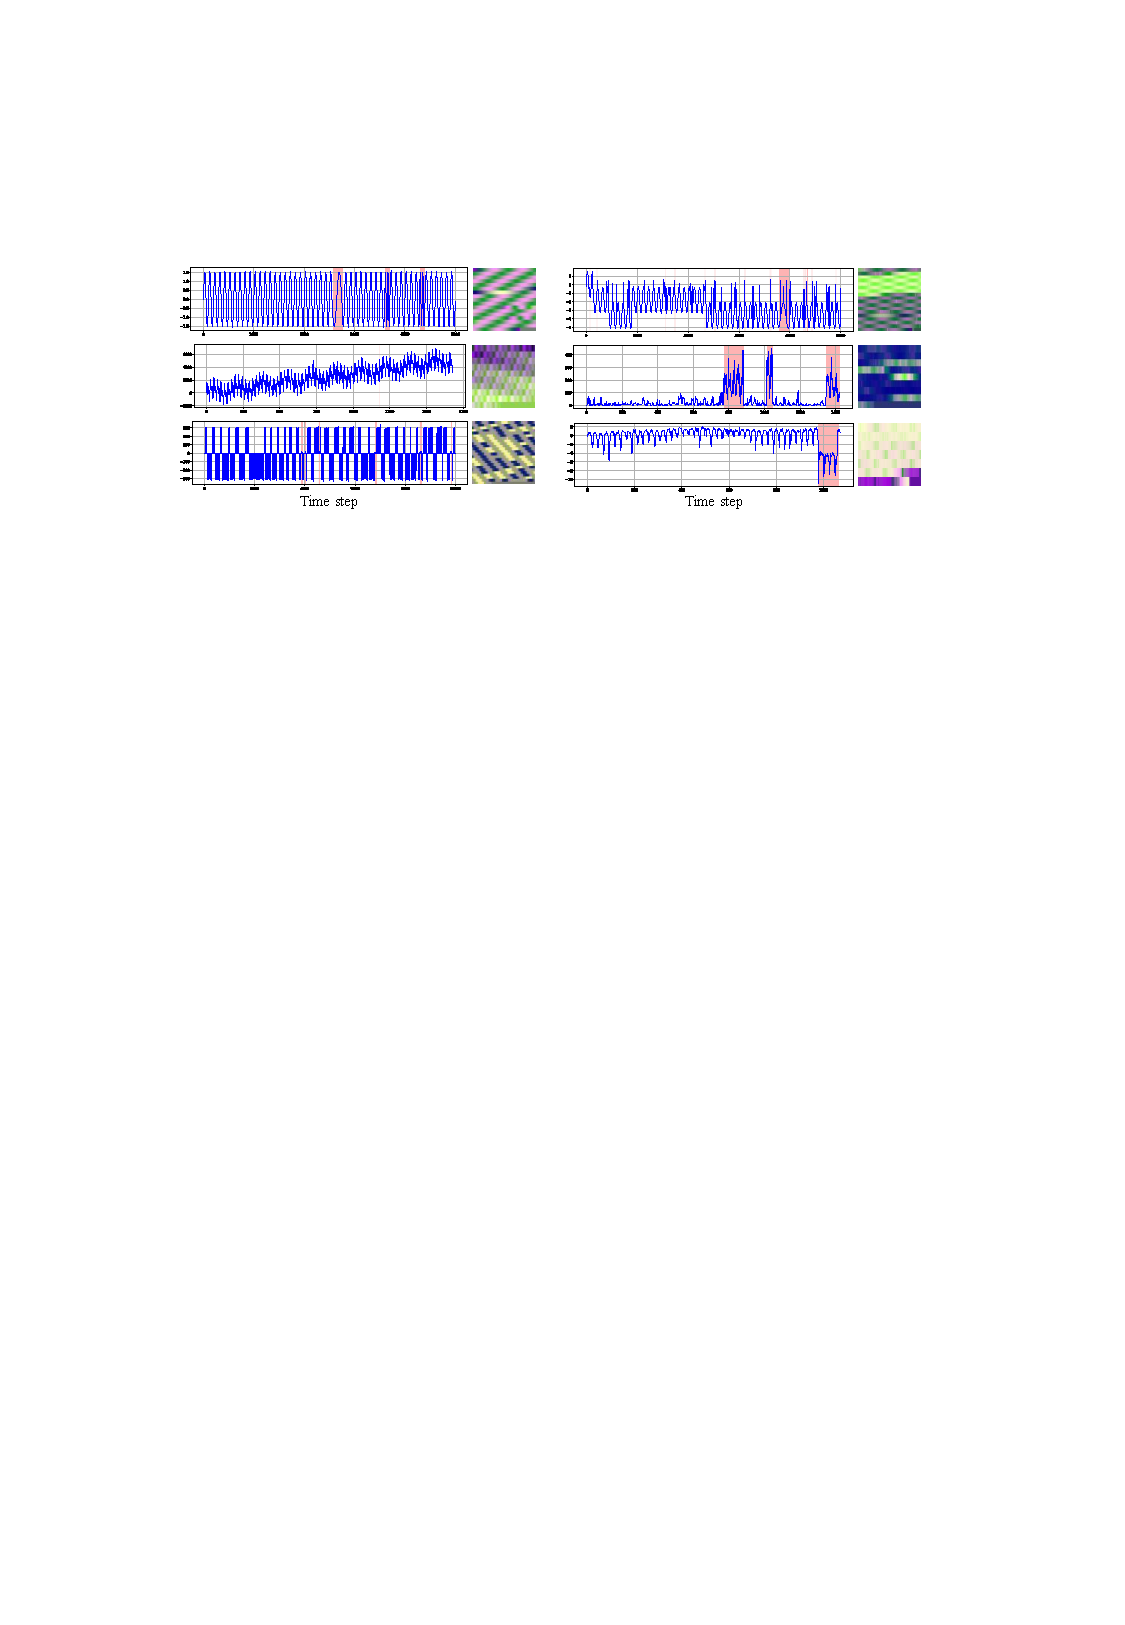
\includegraphics[width=0.9\linewidth]{IMG/img9.pdf}
    \caption{Initial time series and mapping images.}
    \label{fig:img9}
\end{figure}
\begin{figure}[t!]
    \centering
    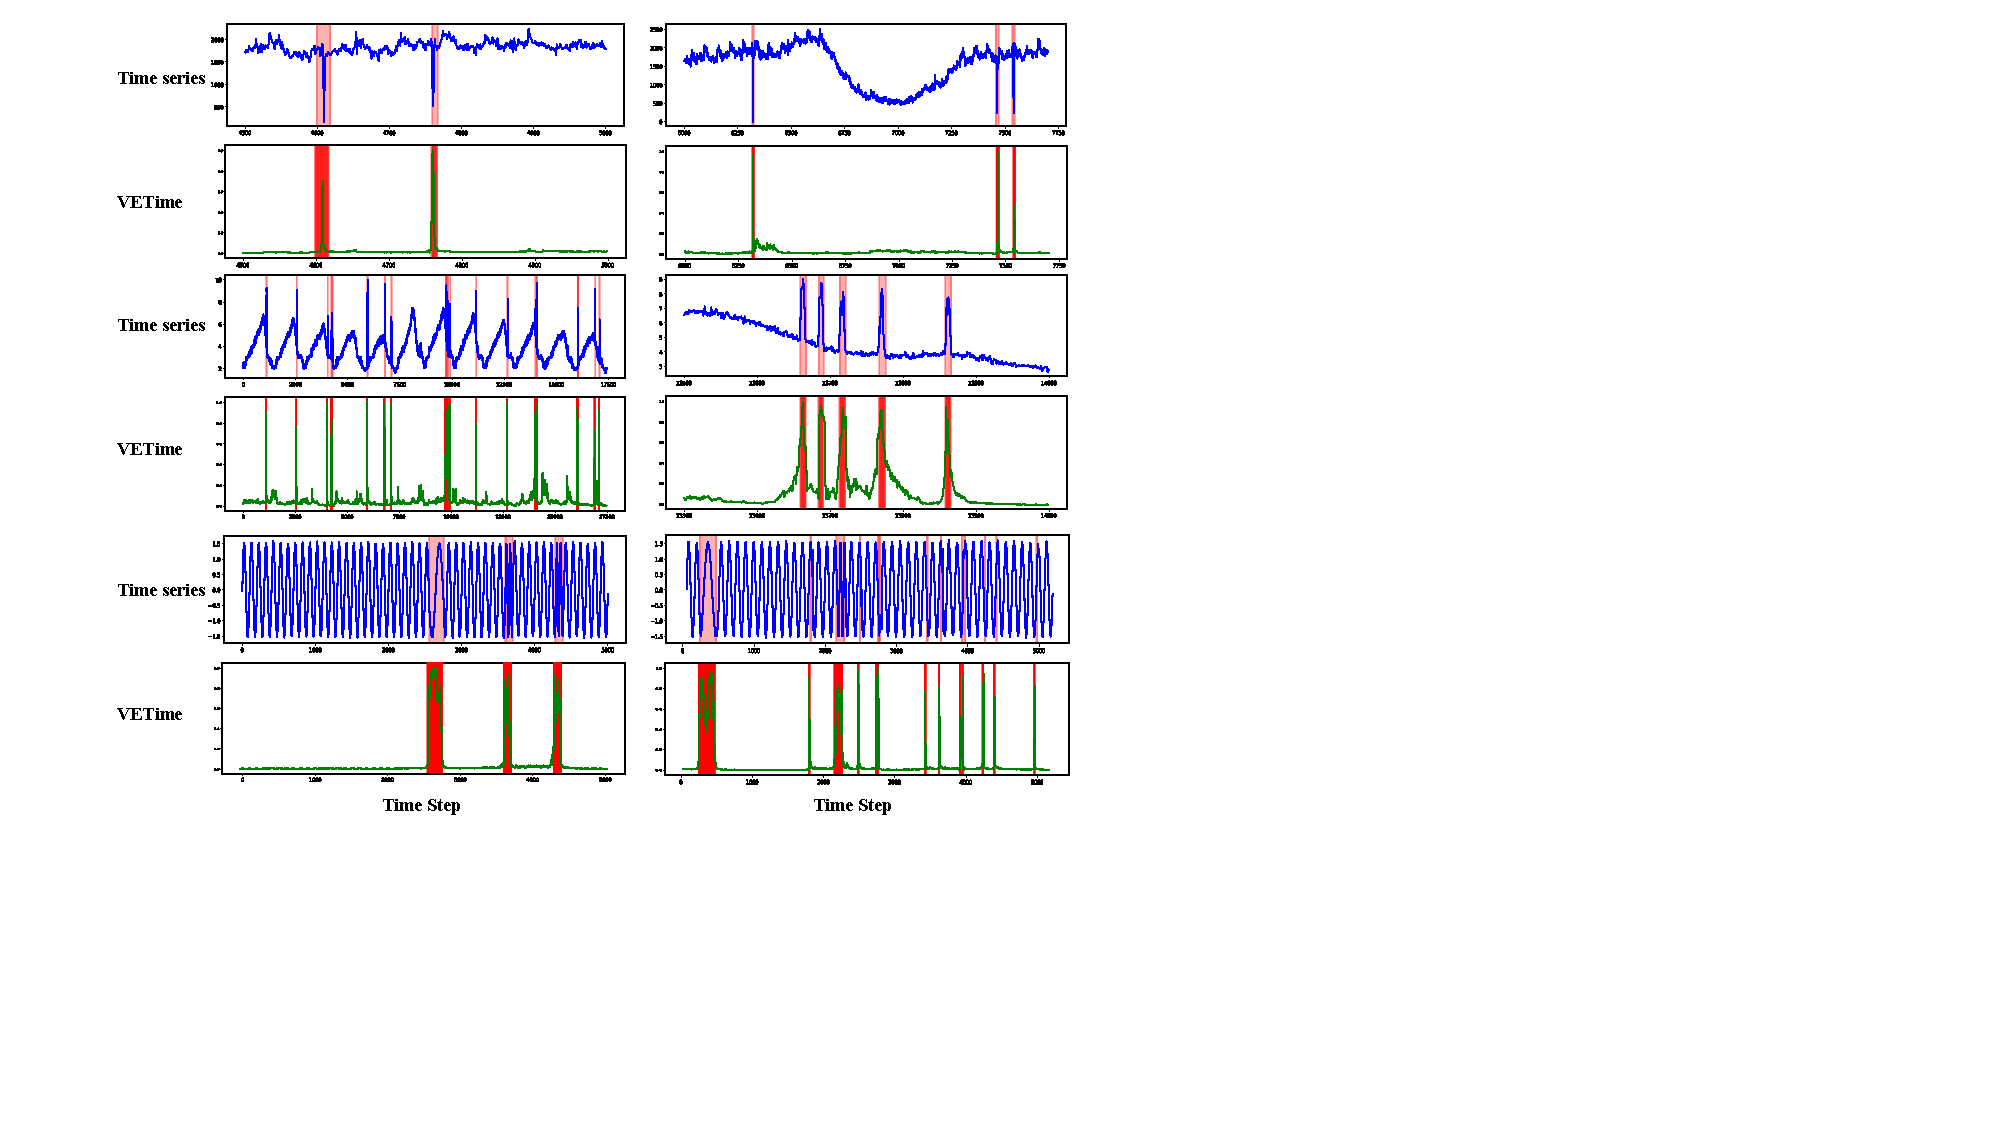
\includegraphics[width=0.9\linewidth]{IMG/img10.pdf}
    \caption{Qualitative visualization of anomaly detection results. Blue curve: original time series; red markers: ground-truth anomaly labels; green curve: predicted anomaly scores.}
    \label{fig:img10}
\end{figure}

\subsection{Comparison under different anomaly types}\label{appendix:C3}
To demonstrate the effectiveness of our method on both global and local anomalies, we categorized and reorganized the NAB and YAHOO datasets into local, global, and mixed anomaly types. Our approach is compared with VIT4TS and TimeRCD, and the results are presented in Table \ref{tab:tab10}. By synergizing the fine-grained sensitivity of temporal features with the global semantic context of visual representations, VETime effectively mitigates the limitations of unimodal baselines and achieve consistent superiority across all anomaly categories.

\section{Visualized results}\label{appendix:D}
\label{appendix:D2}
\subsection{Visualized mappings}\label{appendix:D1}
Figure \ref{fig:img9} visualizes the representations generated by our Reversible Image Conversion module across diverse data samples. The left panels display the raw 1D time-series sequences with ground-truth anomalies highlighted in red, while the right panels present their corresponding 2D visual transformations. As observed, the generated images effectively encode key temporal characteristics, such as periodicity, trends, and noise, into distinct visual textures and patterns. This visualization confirms that our conversion method successfully preserves information-dense global contexts, providing a discriminative basis for the subsequent multi-modal fusion.


\subsection{Visualized anomaly scores}
Figure \ref{fig:img10} presents qualitative anomaly detection results across heterogeneous time series patterns, validating the method's robustness to diverse anomaly patterns. For point anomalies—such as abrupt spikes or isolated dips (visible in Rows 1–2), the green anomaly score curve exhibits sharp, well-localized peaks that precisely align with annotated labels. For context anomalies characterized by extended deviations like sustained trend shifts or contextual drifts (Row 3), the anomaly scores maintain elevated levels throughout the entire anomalous interval, maintaining continuous and coherent alignment with the red-labeled events.



%%%%%%%%%%%%%%%%%%%%%%%%%%%%%%%%%%%%%%%%%%%%%%%%%%%%%%%%%%%%%%%%%%%%%%%%%%%%%%%
%%%%%%%%%%%%%%%%%%%%%%%%%%%%%%%%%%%%%%%%%%%%%%%%%%%%%%%%%%%%%%%%%%%%%%%%%%%%%%%

\end{document}

% This document was modified from the file originally made available by
% Pat Langley and Andrea Danyluk for ICML-2K. This version was created
% by Iain Murray in 2018, and modified by Alexandre Bouchard in
% 2019 and 2021 and by Csaba Szepesvari, Gang Niu and Sivan Sabato in 2022.
% Modified again in 2023 and 2024 by Sivan Sabato and Jonathan Scarlett.
% Previous contributors include Dan Roy, Lise Getoor and Tobias
% Scheffer, which was slightly modified from the 2010 version by
% Thorsten Joachims & Johannes Fuernkranz, slightly modified from the
% 2009 version by Kiri Wagstaff and Sam Roweis's 2008 version, which is
% slightly modified from Prasad Tadepalli's 2007 version which is a
% lightly changed version of the previous year's version by Andrew
% Moore, which was in turn edited from those of Kristian Kersting and
% Codrina Lauth. Alex Smola contributed to the algorithmic style files.

